\documentclass{book}

%margenes del documento
\setlength{\textwidth}{155mm} %longitud horizontal del texto
\setlength{\oddsidemargin}{5mm} %margen del borde frontal
\setlength{\evensidemargin}{7mm}%margen del lomo
\setlength{\topmargin}{-5mm}%margen superior
\setlength{\textheight}{210mm}%altura de texto
\setlength{\parindent}{14pt}

%paquetes usados
\usepackage[utf8]{inputenc}
\usepackage{multicol}
\usepackage{afterpage}
\usepackage{enumerate}
\usepackage{graphicx}
\usepackage{amsmath}
\graphicspath{{./FIguras/}}

\title{Control de conexi\'on a red de parques e\'olicos}
\date{}
\author{Emilio Lia\~no}


\renewcommand*\contentsname{\'Indice}
\renewcommand*\bibname{Referencias}
\renewcommand*\chaptername{Cap\'itulo}

\begin{document}
	\pagenumbering{gobble} %no numera
	%portada
\begin{figure}[h!]
\centering
\includegraphics[width=\textwidth]{Encabezado.PNG}
\end{figure}
\begin{center}
	\LARGE
	UNIVERSIDAD POLIT\'ECNICA DE MADRID \par
	\vspace {10 mm}
	ESCUELA T\'ECNICA SUPERIOR DE INGENIER\'IA Y DISEÑO INDUSTRIAL\par
	\vspace {10 mm}
	\LARGE
	Grado en Ingenier\'ia electr\'onica industrial y autom\'atica \par
	\vspace {10 mm}
	\Huge
	TRABAJO FIN DE GRADO \par
	\vspace{20 mm}
	\LARGE
	\textbf{Control de potencia en el punto conexi\'on a red de parques e\'olicos}\par
	\vspace {10 mm}
	Autor: Emilio Liaño de la Fuente \par
	\vspace {10 mm}
\end{center}
\begin{multicols}{2}
	\LARGE
	Cotutor:

	Manuel Garc\'ia Plaza \par
	Tutor:

	Ricardo Granizo Arrab\'e
\vfill
		
\end{multicols}

\begin{flushright}
\vfill
	Madrid, Julio 2018
\end{flushright}
\afterpage{\null\newpage}
\newpage
\normalsize
\pagenumbering{arabic}

\chapter*{Agradecimientos}

Lo primero quiero agradecer a mi familia, mi gato y mis amigos que siempre han estado mostrando todo su apoyo aun que la situaci\'on se complicara. 

Agradecer a Altran por haberme dado la oportunidad de realizar el trabajo como parte de mi preparaci\'on para el proyecto. Adem\'as a todos mis compañeros de trabajo que siempre estaban dispuestos a ayudarme con cualquier duda, en especial a Manuel, que ha sido cotutor del trabajo y me ha guiado en las partes m\'as oscuras de este recorrido.

Tambien agradecer a Ricardo su labor como tutor resolviendome los problemas tanto acad\'emicos como administrativos derivados de la burocracia universitaria. 

Por ultimo, pero no por ello menos importante, agradecer a la figura de Tesla. Adem\'as de hacer posible la realizaci\'on de este trabajo al descubrir la corriente alterna, es tambien un ejemplo como ingeniero, cient\'ifico y persona en general cuyos pasos siempre he intentado seguir.

\chapter*{Resumen}

Debido a la importancia de la energ\'ia e\'olica en la producci\'on el\'ectrica actual, los c\'odigos de red han adaptado su normativa para permitir la introducci\'on de la potencia instalada a la red de forma estable y segura. Esto significa para los parques e\'olicos la necesidad de implementar un control que cumpla con dicha normativa. \par
En este trabajo se presentan controles de diferentes plantas centr\'andose en garantizar el cumplimiento del procedimiento de operaci\'on 7.4 sobre el control de tensi\'on y reactiva de la red \cite{PO74}. Para ello, se crear\'an modelos de la conexi\'on a red de parques e\'olicos en el entorno de Simulink. \par
Se implementar\'an y analizar\'an casos de estudios para diferentes plantas, diferentes tipos de red y desv\'ios de tensi\'on en el punto de conexi\'on. En el segundo cap\'itulo se describir\'a el funcionamiento de los parques e\'olicos y subconexi\'on a red como introducci\'on a los posibles escenarios que se pueden plantear para su estudio. \par
Se diseñar\'an y aplicar\'an diferentes tipos de algoritmos de control de la potencia activa y reactiva de los generadores modelados. Se comparar\'an las respuestas obtenidas por diferentes tipos de control para el cumplimiento del c\'odigo de red de España. Las diferentes t\'ecnicas utilizadas actualmente y las posibilidades de teor\'ia de control son descritas en el tercer cap\'itulo. \par
Para el modelado del sistema el\'ectrico se utilizar\'an las herramientas de la librer\'ia SimPowerSystem de Simulink. El modelo consta de los elementos t\'ipicos de una conexi\'on a red como las l\'ineas de transmisi\'on, transformadores, generadores y la propia red. En el cuarto cap\'itulo se describen las herramientas usadas de esta librer\'ia y otras de Matlab/Simulink que fueron usadas en este trabajo. \par
Por tanto, los objetivos de este trabajo de fin de grado son la simulaci\'on de un parque e\'olico y presentar diferentes escenarios posibles de conexi\'on a red y la comparaci\'on de diferentes estrategias de control para cumplir los requisitos impuestos por el c\'odigo de red en los diferentes casos anteriormente propuestos. \par

\tableofcontents %indice

\chapter{Introducci\'on}

La importancia de aportar la potencia demandada por la red garantizando una calidad que apoye a la estabilidad de esta es reflejado en los c\'odigos de red que los paises han elaborado para garantizarlo. Las centrales electricas deben cumplir los requisitos impuestos en los c\'odigos de red para poder conectarse a la red. \par

Esta necesidad de cumplir con los criterios impuestos por los c\'odigos de red convierte a los controladores en un elemento imprescindible para el funcionamiento de cualquier planta. En general las condiciones impuestas por los c\'odigos de red son relativas a la potencia activa y reactiva que genera la instalaci\'on por eso los controladores se centran en estas dos factores. \par

La compensaci\'on de reactiva esta asociada a los desfases de tensi\'on que se produce en la red. Los elementos de la red, tanto en el transporte como en el consumo, son principalmente de car\'acter inductivo. Esto genera, normalmente, un aumento en la tensi\'on de la red y de la ocupaci\'on el\'ectrica de las lineas y trasnforamdores. \par

Las plantas genradores son las responsables de evitar esta situaci\'on corrigiendo este desfase desde sus instalaciones. Para ello deben consumir o generar la energ\'ia reactiva como se indica en los c\'odigos de red. Los parques e\'olicos como cualquier otra planta generadora deben colaborar en la compensaci\'on de reactiva. \par

Normalmente este control se apliccaba a nivel individual en cada aerogenerador. En España, este planteamiento era v\'alido para cumplir el RD 2818, que solo tomaba en cuenta el alejamiento del factor de potencia unitario con los datos mensuales. Sin embargo la noramtiva actual requiere un ajuste de precisi\'on que solo se puede conseguir añadiendo una capa de control global regulando el parque al completo. \par

Estos controladores de planta, conocidos como \emph{Power Plant Controller} o PPC, sirven otras funciones a parte de cumplir con las restricciones de las normativas. Son los encargados de maximizar la producci\'on, seguir las instrucciones del operador de red o seguir ciertas pautas que indique el gestor del parque. \par

En el caso de los parques e\'olicos esto suele ser un problema complejo de abordar. El reparto de consignas para un n\'umero variable de generadores, las restricciones de potencia disponible por el viento o las condiciones mediambientales como la parada de m\'aquinas durante las horas de actividad de ciertas especies animales, son problemas que las plantas el\'ectricas cl\'asicas no tenian que tener en cuenta. Por eso en los parques e\'olicos o fotovoltaicos el PPC es una herramienta importante a desarrollar y es la que se ha diseñado en este trabajo. \par 

Como se ha mencionado antes los elementos de la red son de car\'acter inductivo normalmente, esta generalizaci\'on se puede aplicar tambien a los elementos de una planta generadora y en concreto a los de un parque e\'olico. Tanto las m\'aquinas el\'ectricas usadas para la generaci\'on, normalmente m\'aquinas as\'incronas o s\'incronas, como los elementos de transporte, las lineas y los transformadores, son de car\'acter inductivo cuando la planta se encuentra en funcionamiento.\par

Los c\'odigos de red estan escritos teniendo en cuenta esta presunci\'on del car\'acter inductivo en las plantas. Por eso, en ciertos casos, una planta de car\'acter capacitivo podr\'ia compensar m\'as las subidas de tensi\'on dejando a la capacitancia de la planta compensar que siguiendo el c\'odigo de red. \par



	\section{Objetivos}

El objetivo global del trabajo es el diseño y desarrollo de un PCC en el entorno de Matlab/Simulink para controlar la potencia activa y reactiva sumnistrada a la red. Para la consecuci\'on de este objetivo general se han establecido unos objetivos especificos que dicho PCC debe cumplir para poder realizar el estudio de los casos de platnas capacitivas anteriormente mencionados. \par

Como primer objetivo en este trabajo se simular\'a el circuito de conexi\'on a red de un parque e\'olico. En esta fase se debe diseñar un modelo f\'isico de la conexi\'on a red utilizando las herramientas de la librer\'ia \emph{Simscape Power Systems}. Debe incluir como elementos imprescindibles la red, el parque y las lineas de transmisi\'on. \par

De este sistema se deben poder extraer medidas de tensi\'on, intensidad y potencia. Con ellas se verificar\'a el comportamiento de la red y el criterio de signos utilizado en el c\'alculo de la reactiva. Esto es base fundamental para implementar el PPC al ser la realimentaci\'on del control. \par

El segundo objetivo es el diseño de un controlador que sea capaz de cumplir el c\'odigo de red de España. En concreto cumplir con lo establecido en el procedimiento de operaci\'on 7.4 referente a compensaci\'on de reactiva ante variaciones de tensi\'on. \par

Para considerar cumplido este objetivo la planta tendra que seguir la consigna de reactiva sin salirse de los margenes establecidos por la normativa española ante diferentes tipos de variaciones de tensi\'on en la red como el escal\'on, la rampa o la sinusoidal. Adem\'as el control debe actuar siguiendo estas entradas en todos los casos de estudio propuestos, tanto para las difernetes potencias nominales como para las plantas inductivas y capacitivas. \par

Por \'ultimo los efectos de aplicar o no la compensaci\'on de reactiva que se establece en el c\'odigo de red para los diferentes casos de estudio del car\'acter de la planta. Teniendo en cuenta que el c\'odigo de red esta escrito suponiendo que las plantas generadoras son de car\'acter inductivo, las plantas que son de car\'acter capacitivo podr\'ian compensar mejor las subidas de tensi\'on con las propias caracteristicas de la planta que siguiendo la normativa. \par

Se comparar\'a como actuan diferentes plantas propuestas en los casos de estudio ante la subida de tensi\'on provocada la inyecci\'on de potencia activa en la red. Dependiendo de la cantidad de potencia activa que se genere tambien habra diferentes casos de estudio puesto que la tensi\'on variara en funci\'on de la intensidad que entregue la planta a la red. \par


\chapter{Parques e\'olicos y conexi\'on a red}

Un parque e\'olico es una agrupaci\'on de aerogeneradores que transforman la energ\'ia e\'olica en energ\'ia el\'ectrica. En este cap\'itulo se har\'a una introducci\'on a los elementos de un parque e\'olico prestando especial atenci\'on a los elementos el\'ectricos y de control. Primero se expondran los elementos en general de un parque e\'olico y de la conexi\'on a la red, despu\'es se hablar\'a de los parametros el\'ectricos del circuito de conexi\'on y de su comportamiento, y por \'ultimo se hablar\'a de los c\'odigos de red y de las limitaciones que estos inponen sobre el funcionamiento de los parques e\'olicos.  

	\section{Elementos del parque}
Los parques e\'olicos necesitan para su funcionamiento los aerogeneradores para transformar la energ\'ia e\'olica en energ\'ia el\'ectrica, un sistema de control central y una red interna para la conexi\'on el\'ectrica. A su vez estos est\'an compuestos por diferentes elementos.

		\paragraph{Aerogenerador}
		Los aerogeneradores funcionan convirtiendo la energ\'ia cin\'etica del viento en energ\'ia mec\'anica rotatoria y esta, en energ\'ia el\'ectrica en una m\'aquina trif\'asica. Hay dos tipos seg\'un la disposici\'on de sus aspas, los de eje horizontal y los de eje vertical. A nivel industrial la impuesta es el eje horizontal por su rendimiento, fiabilidad y la capacidad de adaptarse a diferentes potencias. Este tipo de aerogenerador consta de un rotor, una multiplicadora, un generador trif\'asico, la conexi\'on a la red y un sistema de control. \par
		El rotor tiene las aspas que normalmente son tres, se puede variar la orientaci\'on de las palas en funci\'on de la velocidad del viento o de la potencia deseada. La multiplicadora transforma la baja velocidad y alto par del eje del rotor en alta velocidad y un par bajo en el eje del generador el\'ectrico, no todos los modelos lo incluyen necesariamente pero su uso est\'a muy extendido. El generador trif\'asico puede ser s\'incrono  o as\'incrono, esto depende de la topolog\'ia de conexi\'on que se utilice.  \par
		La conexi\'on a red se puede hacer de forma directa, para lo que se utiliza un generador as\'incrono de jaula de ardilla. Este tipo de conexi\'on se conoce tambi\'en como conexi\'on de velocidad fija porque la velocidad del rotor depende directamente de la frecuencia de la red, que normalmente es fija. En este sistema, a pesar de lo robusto que es por su sencillez se necesitan resistencias rot\'oricas para aumentar el rango de velocidades del viento con las que se puede trabajar, adicionalmente hay que incluir un banco de condensadores para compensar la potencia reactiva, ocasionando posibles resonancias en la red \cite{TopologiasWT}. \par 
		Otro tipo de conexi\'on es la doblemente alimentada, para esta configuraci\'on tambi\'en se usan m\'aquinas as\'incronas. En esta topolog\'ia el estator se encuentra conectado de forma directa a  la red como encontr\'abamos antes, pero el rotor est\'a conectado tambi\'en a la red por medio de un circuito de electr\'onica de potencia, consistente de un convertidor AC-DC-AC ‘back to back’ \cite{AerogeneradorDIFG}. Este tipo de topolog\'ia aumenta el rango de velocidades para generar potencia activa, la velocidad m\'axima estar\'a limitada a la potencia del convertidor, adem\'as permite tener un control sobre el factor de potencia de la m\'aquina, requisito necesario para poder conectarse a la red el\'ectrica. \par
		Por \'ultimo, la tercera topolog\'ia de conexi\'on normalmente utilizada es la \emph{‘Full Converter’}. Con este tipo de conexi\'on a la red se suelen utilizar m\'aquinas s\'incronas. En esta conexi\'on el estator est\'a conectado a la red a trav\'es de un convertidor ‘back to back’, sin ninguna conexi\'on adicional. En cuanto al rango de velocidades y el control de reactiva ofrece car\'acter\'isticas parecidas al doblemente alimentado, pero existen diferencias en coste. El doblemente alimentado es m\'as barato que el \emph{‘Full Converter’} inicialmente pero necesita un mantenimiento m\'as caro y ofrece menos potencia de salida anual \cite{PMGvsDFIG}. Ambos dos requieren un controlador de los transistores IGBT para su funcionamiento que los hace m\'as sofisticados.  \par
		Adem\'as del control de la salida el\'ectrica hay un controlador en cada torre para asegurar la seguridad y eficiencia del aerogenerador a nivel mec\'anico y aerodin\'amico. Por medio de m\'odulos para el control de equipos de potencia, el controlador de la turbina recibe la informaci\'on de los par\'ametros monitorizados y manipula los interruptores, bombas hidr\'aulicas, v\'alvulas y motores para controlar dichos par\'ametros. Estos controladores a su vez se comunican con un controlador central de todo el parque \cite{ComunicationControl}.  \par

		\paragraph {Controlador}
		El sistema de control de la planta incluye el propio controlador, la comunicaci\'on interna del parque y el SCADA, \emph{Supervisory Control And Data Acquisition} en español Supervisi\'on, Control y Adquisici\'on de Datos, para operar el sistema. Debido al aumento de los parques e\'olicos con una gran potencia y su penetraci\'on en la red, es necesario que estos se comporten como componentes activos controlables de la red apoyando su estabilidad. Para eso es necesario instalar un sistema de control central del parque. Este control es responsable de que el parque funcione de forma segura, \'optima y cumpliendo los reglamentos impuestos por la red el\'ectrica a la que este alimentando. \par
		Uno de los principales requerimientos que se especifican en la normativa del parque est\'a referido a los huecos de tensi\'on en la red. El objetivo es evitar la p\'erdida significativa de producci\'on de los aerogeneradores a lo largo de la duraci\'on de la falta. Los requerimientos de control se refieren a diferentes aspectos de la potencia del sistema y la estabilidad. \par 
		Dependiendo del estado de la red, el operador del sistema realiza demandas espec\'ificas al control central del parque, el cual prepara las señales de consigna a cada aerogenerador en concreto. El controlador central se encarga de cumplir los requerimientos del operador de red mandando las referencias de potencia activa y reactiva que se necesita de cada aerogenerador. Estas consignas se calculan con las medidas obtenidas en el PCC, \emph{Point of common coupling} en español punto de acoplamiento com\'un, y con la potencia disponible que ofrece cada rotor \cite{WindFarmController}.  \par
		La red de comunicaci\'on del parque est\'a formada por los controladores de los aerogeneradores, que est\'an instalados en la torre de cada turbina, que se comunican con el controlador central.  A su vez los controladores de cada torre recogen toda la informaci\'on necesaria de los modulos, que est\'an conectados con los instrumentos de medida a trav\'es de  un sistema de sensores. Los controladores de los aerogeneradores mandan toda la informaci\'on al controlador central y asignan las consignas que manda este a los modulos dentro del aerogenerador \cite{ComunicationControl}.  \par
		Adem\'as de los modulos instalados en cada turbina, la red de control cuenta con diferentes modulos conectados al controlador central. Entre otros el modulo de la l\'inea, el del trasformador, los de los buses de comunicaci\'on y los conectados a las redes de alimentaci\'on de los aerogeneradores. Estos modulos monitorizan las condiciones de operaci\'on como los desequilibrios de tensi\'on, el sobrecalentamiento, fases inversas, sincronizaci\'on pobre y los l\'imites de tensi\'on y frecuencia\cite{ComunicationControl}.   \par
		La red t\'ipica de un sistema de comunicaciones consiste de una conexi\'on principal de amplio ancho de banda y redes de bajo ancho de banda conectadas individualmente a la principal. La fibra \'optica y las microondas de radio suelen ser las tecnolog\'ias usadas para la comunicaci\'on principal. En las redes secundarias se suele utilizar cable de par trenzado de cobre, aunque se pueden usar tambi\'en sistemas inal\'ambricos. Generalmente en el caso de los parques e\'olicos se suelen utilizar PLCs, \emph{Power Line Communications} en español comunicaci\'on por l\'inea de potencia. Las tecnolog\'ias de PLCs disponibles permiten una gran velocidad transmisi\'on llegando a los 200 Mb/s. La principal ventaja de este tipo de comunicaci\'on es que las señales viajan a trav\'es de los mismos cables de la l\'inea el\'ectrica. Por otro lado estos cables suelen estar desprotegidos contra interferencias electromagn\'eticas y los m\'odulos que utilizan son m\'as caros que los de la comunicaci\'on inal\'ambrica \cite{ComunicationWF}. \par
	
	\section{Elementos de la conexi\'on a red}
	
	La red del parque est\'a formada por l\'inea de media tensi\'on que conecta con todos los aerogeneradores, la l\'inea de alta tensi\'on que conecta con la red el\'ectrica general a la que se le aporta la potencia y una subestaci\'on que contiene varios elementos. El PCC est\'a a un lado del transformador, dependiendo de si las medidas se toman del lado de baja o de alta tensi\'on es el criterio utilizado para dictaminar donde est\'a el PCC. \par
		\paragraph {L\'ineas de transmisi\'on}
Las l\'ineas de media tensi\'on generalmente en los parques conectan todos los aerogeneradores con el transformador con diferentes topolog\'ias. Las formas de conectar las l\'ineas de alimentaci\'on de los aerogeneradores son numerosas pero generalmente se utiliza la radial, la radial bifurcada, la de alimentaci\'on-subalimentaci\'on y en bucle. \par

La conexi\'on radial consiste de un solo cable de alimentaci\'on que se conecta secuencialmente a todos los aerogeneradores del parque, es la m\'as simple y por tanto la m\'as barata, es la que mejor se adapta para parques con los aerogeneradores en l\'inea. La radial bifurcada es parecida a la radial pero la l\'inea se divide para poder alimentar a dos series de aerogeneradores en paralelo, es la m\'as barata pero un fallo en la l\'inea supone una p\'erdida de todos los aerogeneradores. La alimentaci\'on-subalimentaci\'on junta varios cables de alimentaci\'on en radial en uno principal manteniendo los elementos de seguridad de cada cable de alimentaci\'on secundario, generalmente se usan para parques de gran tamaño que est\'an distribuidos en una gran \'area. La topolog\'ia en bucle conecta todos los cables secundarios de alimentaci\'on secundarios para evitar que un fallo en una de las l\'ineas la deje inoperante, es la m\'as segura de todas las topolog\'ias \cite{ComunicationTopologies}.\par
		\paragraph {Subestaci\'on}
El cable de alimentaci\'on general llega a la subestaci\'on donde se transforma la media tensi\'on en alta con un transformador. Dentro de la subestaci\'on, adem\'as de los componentes de los lados de media y alta tensi\'on, podemos encontrar los sistemas de medida y control, sistemas de protecci\'on contra incendios u otras incidencias y un sistema para ajustar la potencia reactiva. Tradicionalmente este sistema consistia de un sistema mecanico de bajo coste que conectaba un banco de condensadores. A pesar de que estos dispositivos ayudan a mejorar el factor de potencia y la regulaci\'on de tensi\'on en estado estacionario, no se puede resolver satisfactoriamente problemas como las fluctuaciones de potencia o tensi\'on y la eliminaci\'on de harm\'onicos. \par

La integraci\'on de los aprque e\'olicos a la red requiere una compensaci\'on de la potencia reactiva din\'amica para apoyar a la estabilidad, sobre todo durante perturbaciones en la red. Para conseguir un alto rendimiento en el control de la tensi\'on tanto en transitorio como estacionario en el PCC se utilizan FACTS, \emph{flexible ac transmission system} en español sistema flexible de transmisi\'on en corriente alterna. Los dos m\'as comunes usados en parques e\'olicos son el SVC, \emph{static var compensator}, y el STATCOM, \emph{static synchronous compensator} \cite{FACTS}.  \par

El STATCOM suele ser la opci\'on considerada para esta soluci\'on por las ventajas que presenta frente al SVC. Entre estas ventajas se encuentra un tiempo de respuesta m\'as r\'apido y una capacidad de aporte de tensi\'on auxilair mayor por su naturaleza de fuente de tensi\'on \cite{STATCOM}. \par

En el lado de media tensi\'on se suele encontrar el barraje que conecta la red al cuadro el\'electrico, el seccionador para abrir el circuito cuando no hay corriente y un interruptor autom\'atico para abrir el circuito ante corrientes el\'ectricas elevadas. En el lado de alta tensi\'on suele haber reactancia a tierra en los transformadores, una toma a tierra general, descargadores de sobretensi\'on, otro seccionador y otro disyuntor.  \par


	\section{Par\'ametros de la red trif\'asica} 
	
	Todas las l\'ineas el\'ectricas descritas en la secci\'on anterior son trif\'asicas por las ventajas que este tipo de redes presentan frente a las monof\'asicas. En esta secci\'on se cubrir\'an todos los par\'ametros que hay que controlar de una red trif\'asica, su sentido f\'isico y las ecuaciones que los relacionan. \par

El circuito que se va a analizar se puede reducir a una fuente de intensidad, que ser\'ia el conjunto de aerogeneradores. Una l\'inea que une esta fuente con el primario del transformador y otra l\'inea que une el secundario con la red. Finalmente, la red estar\'ia representada por una fuente de tensi\'on. En los parques e\'olicos reales las medidas de los par\'ametros de la red solo se realizan a un lado del transformador, pero para analizar el circuito en esta secci\'on se colocaran medidores a ambos lados. Los par\'ametros de la red que se observan y controlan en un parque e\'olico son la tensi\'on, la intensidad, la potencia, tanto activa, reactiva y aparente y la frecuencia. \par

Para la medici\'on de estos valores se considera que los circuitos de la red de conexi\'on son equilibrados, por lo que las tensiones de cada fase y las intensidades tendr\'an el mismo valor eficaz y un desfase de 120º entre s\'i. Para expresar esta diferencia de fase se suele utilizar la notaci\'on fasorial,  pero por la simplicidad a la hora de hacer ciertos c\'alculos como la suma o la resta se usan n\'umeros complejos para definir los vectores tambi\'en. Para poner una referencia a la fase se le da a un valor de tensi\'on o corriente el valor 0 o 90 de fase. En este caso, para tomar el mismo crit\'erio que los resultados de Simulink, se dar\'a fase 0 a la intensidad de la primera fase, $I_a$. \par

Las fuentes de intensidad generan tres ondas sinusoidales de igual amplitud y desfasadas entre ellas 120º. Conectada a una carga se pueden observar tambien tres ondas sinusoidales de voltage que tambi\'en son equilibradas. Entre las ondas de tensi\'on e intensidad existe una relaci\'on dada por la impedancia de la carga representada en la ley de Ohm. \par

\begin{equation}\label{eq:ohm}
	\overline{I}=\overline{V}/\overline{Z}
\end{equation} \par

Donde $\overline{I}$ es la intensidad que circula por la impedancia, $\overline{V}$ es la caida de tensi\'on en se produce en la impedancia y el valor de la impedancia esta representado por $\overline{Z}$. \par

Si los par\'ametros de la ecuaci\'on son introducidos como fasores y teniendo en cuenta que la fase de la intensidad se considera 0, podemos concluir que el desfase entre la intensidad y la tensi\'on viene dado por la fase de la carga y la relaci\'on entre los m\'odulos es el m\'odulo de la impedancia. Si la impedancia es puramente resistiva el desfase es nulo entre ambas, si es de car\'acter capacitivo la intensidad va adelantada y si es de car\'acter inductivo la intensidad va retrasada respecto a la tensi\'on. \par

Para observar este efecto de la carga sobre la relaci\'on entre tensi\'on e intensidad se simula el circuito de la figura \ref{LoadAnalyserModel} y cambiando los valores de la impedancia se obtienen las gr\'aficas de la figura \ref {Va_IaALL}, en las que se puede ver en el transitorio como la intensidad de la primera fase, $I_a$,  se adelanta o se retrasa respecto a la tensi\'on, $V_a$, dependiendo del tipo de carga.  \par

\begin{figure}[h!]
\centering
\includegraphics[width=0.9\textwidth]{LoadAnalyserModel.PNG}
\caption{Modelo de una carga alimentada por una fuente de intensidad trif\'asica en Simulink}
\label{LoadAnalyserModel}
\end{figure}

\begin{figure}[h!]
\centering
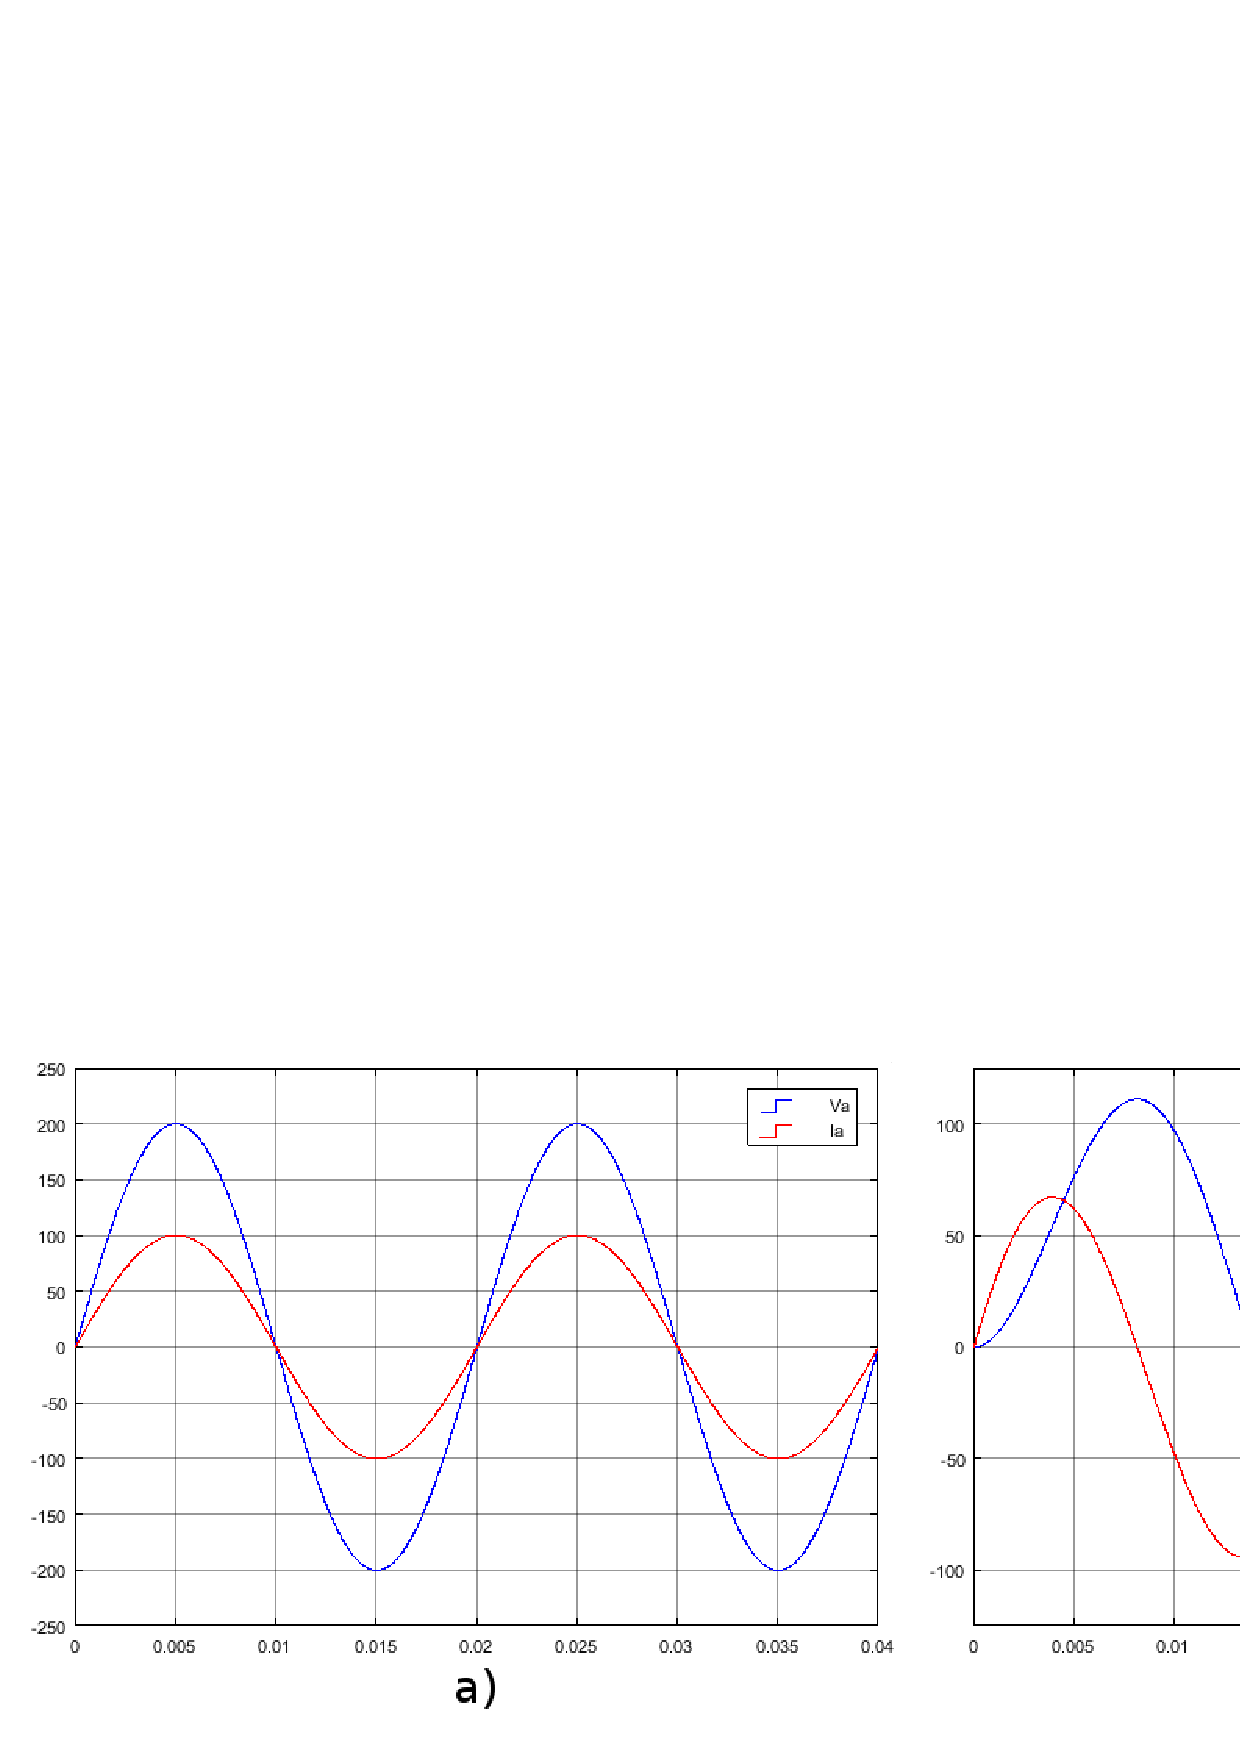
\includegraphics[width=1\textwidth]{Va_IaALL.PNG}
\caption{Respuesta del circuito ante carga resistiva a), capacitiva b) e inductiva c).}
\label{Va_IaALL}
\end{figure}

Cuando la carga es puramente capacitiva o inductiva se produce un desfase entre la intensidad y la tensi\'on de 90º. Si la carga es capacitiva, al estar la intensidad adelantada respecto a la tensi\'on el angulo visto desde la tensi\'on sera positivo y si la carga es inductiva el angulo sera negativo visto desde la tensi\'on como se puede ver en la figura \ref {PhasComp}. Para todos los calculos de potencias el angulo se ve desde la tensi\'on a la intesidad, por eso se utiliza ese criterio de signos. \par

\begin{figure}[h!]
\centering
\includegraphics[width=1\textwidth]{PhasComp.PNG}
\caption{Fasores de una carga puramente capacitiva a) e inductiva b).}
\label{PhasComp}
\end{figure}

En el an\'alisis de la conexi\'on a red es importante la potencia, esta debe cumplir con los requisitos que marcan el operario de red y el c\'odigo de red. Para el c\'alculo de la potencia de una red trif\'asica se utiliza la siguiente f\'ormula:   \par

\begin{equation}
	\overline{S}=\sqrt{3} \overline{V}_L  \overline{I}_L^*
\end{equation} \par

Podemos observar que la potencia consumida o sumisnistrada por un elemento del circuito tiene una componenente real y una componenente imaginaria que se llaman potencia activa, $P$ y reactiva, $Q$ respectivamente. Desarrollando la formula anterior usando su representaci\'on en n\'umeros complejos llegamos a lo siguiente: \par

\begin{equation}\label{eq:potensia}
	\overline{S}= \sqrt{3} V_L I_L \cos{\varphi}+j\sqrt{3} V_L I_L \sin{\varphi} = P+jQ 
\end{equation} \par

Donde $\varphi= \alpha_V-\alpha_I$, la diferencia entre el angulo de la tensi\'on y el angulo de la intensidad. Por lo tanto basandose en el criterio de signos anteriormente mencionado para los \'angulos trataremos la $Q$ negativa como capacitiva y con signo positiva como inductiva. \par

\'Analizando la diferencia de tensi\'on entre dos puntos de un circuito que esta descrita por la ecuaci\'on (\ref{eq:ohm}), donde la tensi\'on antes de la carga es $E$ y la tensi\'on despues de la carga es $V$ tenemos que:

\begin{equation}\label{eq:difV}
	\Delta V=E-V=ZI
\end{equation} \par

 Despejando la ecuaci\'on (\ref{eq:potensia}) en la ecuaci\'on (\ref{eq:difV}) obtenemos el siguiente desarrollo:

\begin{equation}\label{eq:lol}
	\Delta V=(R+jX)\frac{P-jQ}{E}= \frac{RP+XQ}{E}+j\frac{XP-RQ}{E}
\end{equation} \par

Cuando hablamos de una linea de transmisi\'on, como son las que conectan el parque con al subestaci\'on y esta con la red, consideramos que $X \gg R$ \cite{WFgridcode}. Considerando entonces despreciable el valor de $R$ en la formula (\ref{eq:lol}) queda lo siguiente: 

\begin{equation}
	\Delta V= Q\frac{X}{E}+jP\frac{X}{E}
\end{equation} \par

Esto significa que los cambios en la magnitud de de la tensi\'on son controlados por la potencia reactiva y la  diferencia de fase entre emisor y receptor viene dada por la potencia activa \cite{WFgridcode}. Por eso se utiliza el control de la potencia activa y reactiva para controlar frecuencia de la red y la tensi\'on respectivamente. \par

Normalmente la fercuencia es m\'as estable que la tensi\'on en la red el\'ectrica por lo que los parques e\'olicos tratan de producir la potencia el\'ectrica m\'axima que permita la instalaci\'on y la demanda de la red, y as\'i obtener los mayores beneficios posibles. Es por eso que ante las variaciones de tensi\'on en la red se var\'ia la potencia reactiva entregada o consumida manteniendo la potencia activa. \par


	\section{C\'odigos de red}

Un c\'odigo de red es un conjunto de especificaciones t\'ecnicas que definen los par\'ametros que debe cumplir una instalci\'on para asegurar la seguridad y estabilidad de la red p\'ublica a la que est\'a conectada  \cite{UKgridCode}. Dichas instalaciones pueden ser plantas el\'ectricas generadoras, consumidores u otra red. En este apartado se prestara especial atenci\'on a los c\'odigos de red referidos a plantas el\'ectricas y al c\'odigo de red de España en concreto. \par

Los c\'odigos de red var\'ian seg\'un la red para la que se han diseñado. Es por eso cada pa\'is tiene un c\'odigo de red propio, pero no solo var\'ia de un pa\'is a otro sino que incluso dentro de España las condiciones que se imponen en la red peninsular o no peninsulares son distintas por las diferencias en las redes y las condiciones en las que operan. A pesar de las diferentes restricciones, los casos que se abordan en los c\'odigos de red suelen ser comunes para la mayor\'ia de ellos.  \par

Un ejemplo de esta variaci\'on es el tratamiento de las perdidas de tensi\'on en la red. En la figura \ref{FaultGCs} se puede ver la comparativa de especificaciones entre los diferentes c\'odigos de red europeos para la respuesta temporal de la tensi\'on ante una caida. \par

\begin{figure}[h!]
\centering
\includegraphics[width=0.8\textwidth]{FaultGCs.PNG}
\caption{Respuesta de tensi\'on ante caida en los c\'odigos de red europeos \cite{FaultGC}.}
\label{FaultGCs}
\end{figure}

En el caso de la conexi\'on y operaci\'on de plantas generadoras los requerimientos m\'as importantes para el control son los rangos de frecuencia y tensi\'on, el control de la potencia activa y el control de la reactiva en operaci\'on normal. Tambien se cubren los casos de perturbaciones en la red como los huecos de tensi\'on o la inyecci\'on de corriente reactiva. Normalmente estos requerimientos pueden ser descritos en las siguientes zonas de operaci\'on para frecuencia y tensi\'on: Operaci\'on continua en un rango limitado alrededor del punto nominal, operaci\'on por tiempo limitado con una posible reducci\'on de la salida en unos margenes extendidos y por \'ultimo la desconexi\'on inmediata \cite{GridCodeDeepAnalisys}.\par

		\paragraph{Tensi\'on}
Respecto al control de tensi\'on, en la secci\'on anterior se ha visto que la magnitud de la tensi\'on esta controlada por la potencia reactiva. Por lo tanto el control de la tensi\'on se expone en los c\'odigos de red como un control de la potencia reactiva en funci\'on de la tensi\'on de red \cite{WFgridcode}. \par

En los PO, procedimientos de operaci\'on que forman el c\'odigo de red de España, el control de la potencia reactiva esta definido por la potencia activa neta instalada del parque. En el PO 7.4 \cite{PO74}  se establece que todos los generadores deben funcionar dentro de el margen de generaci\'on/absorci\'on que aparecen en la figura \ref{VQgridcode}.   \par 

\begin{figure}[h!]
\centering
\includegraphics[width=0.8\textwidth]{VQgridcode.PNG}
\caption{L\'imites de potencia reactiva en funci\'on de la tensi\'on de la linea}
\label{VQgridcode}
\end{figure}

Para comprobar que se cumplen los requisitos de tensi\'on y potencia reactiva se hacen controles de estos valores cada cinco minutos por parte del operador del sistema. Se establece una banda admisible de $\pm2.5 kV$ entorno al valor de consigna. Se considera un servicio adecuado cuando se cumple al menos un $75\%$ de los valores muestreados cada hora. Para cumplir con los valores la tensi\'on  se debe mantener dentro de los margenes admisibles de variaci\'on o la central debe haber alcanzado el limite de potencia reactiva obligatorio \cite{PO74}. \par

		\paragraph{Frecuencia}
Como consecuencia de un desajuste entre la potencia activa aportada y la demanda se produce un cambio en la energía almacenada en la masa rotativa del generador que provoca un desvio de la frecuencia del sistema. Un aumento en la potencia entregada se convertir\'ia en un aumento de la velocidad angular del generador y por tanto un aumento de frecuencia, pasando lo contrario al entregar potencia por debajo de la demanda \cite{WFgridcode}, \cite{FrecuencyLvL}. \par

Normalmente el control de la frecuencia esta compuesto por tres funciones distintas. El control primario de frecuencia, usado ante los desequilibrios repentinos en la red. Actua a nivel local en la turbina en un rango de 15 a 30 segundos. El control secundario o de carga permite reestablecer la frecuencia y la potencia a los valores programados. Se realiza en las unidades de control central del parque y actua en un rango de 15 minutos. Este es el tipo de funci\'on que se implementara en este trabajo. Finalmente esta el control terciario que consiste en la gesti\'on de la potencia generada por cada aerogenerador para ayudar al control secundario \cite{WFgridcode}. \par

En el PO 1.5 se trata el establecimiento de la reserva para la regulacion de frecuencia y potencia. Respecto al control primario, se especifica que debe completar un reestablecimiento total antes de 15 segundos desde el instante de desequilibrio si el valor de esre es menor o igual a 1500 MW. En caso de que el desequilibrio sea superior a 1500 MW el 50\% la reserva de regulaci\'on primaria debe actuar antes de 15 segundos y se debe alzanzar el 100\% de actuaci\'on antes de 30 segundos. La regulaci\'on primaria debe actuar durante un tiempo de 15 minutos hasta que la regulaci\'on secundaria recupere las consignas iniciales y reestablezca la reserva primaria utilizada \cite{PO15}. \par

La actuaci\'on de la reserva secundaria no debe retarserse m\'as de 30 segundos y debe mantenerse durante un tiempo de 15 minutos hasta que su uso neto sea sustituido por la regulaci\'on terciaria. Se deben garantizar unos valores m\'inimos de reserva de 500 MW a subir y 400 MW a bajar. Sobre la reserva terciaria se dice que se ha de mantener unos margenes de subida y bajada de potencia para prevenir las diferencias de demanda real con respecto a la esperada y de la producci\'on de las centrales e\'olicas respecto a la esperada \cite{PO15}. \par

Por otra parte, en el PO 1.2 se especifican los limites de frecuencia admisibles del sistemas y las correciones que se deben aplicar de potencia activa. Estando los limites de subfrecuencia entre $49,8Hz$ y $49,5Hz$, y de sobrefrecuencia en $50,2Hz$ y $50,5Hz$. Para estos limites la correcci\'on de potencia activa se rige por la ecuaci\'on (\ref{eq:PF}) que devuelve difrenecia de potencia, $\Delta P$, a imponer respecto a la referencia, $P_{ref}$ \cite{PO12}. \par

\begin{equation}\label{eq:PF}
	\frac{\Delta P}{P_{ref}}=100 \frac{\frac{|\Delta f|-|\Delta f_1|}{f_n}}{s_2}
\end{equation} \par

Donde $\Delta f_1$ es la difrencia de frecuencia entre la tensión nominal, $f_n$, de $50Hz$ y los limites fijados por el c\'odigo de red m\'as cercanos a $f_n$ segun el caso sea de sobrefrecuencia o subfrecuencia. Adem\'as $s_2$ es el estatismo en porcentaje que debera ajustar a un rango entre 2\% y 12\% \cite{PO12}. \par

En la figura \ref{FPgridcode} se muestran los limites de $\Delta P$ que se pueden imponer en funci\'on de los valores limites para $s_2$. Los valores validos son aquellos que se encuentran en el area comprendida entre las dos rectas. 

\begin{figure}[h!]
\centering
\includegraphics[width=0.65\textwidth]{FPgridcode.PNG}
\caption{L\'imites de variaci\'on de potencia activa en funci\'on de la desviaci\'on de frecuencia}
\label{FPgridcode}
\end{figure}

En este mismo documento se especifica que las tecnolog\'ias cuya energ\'ia primaria sea renovable y se conecten a la red mediante convertidores electr\'onicos, como es el caso de los aerogeneradores modernos y por extensi\'on de la mayor\'ia de parques e\'olicos, se contribuira a la maximizaci\'on de producci\'on y se minimizara la necesidad de aplicar limitaciones a su producci\'on. Esto significa que este control podr\'a desactivarse siempre que el operador del sistema considere que existen otros medios para evitar poner en riesgo la calidad del suministro, pero es necesario que se pueda activar en tiempo real si as\'i se solicitase \cite{PO12}. \par

\chapter{Control de plantas el\'ectricas}

La teor\'ia de control es un campo de la ingenier\'ia y las matem\'aticas que trata el comportamiento de los sistemas din\'amicos. El problema de control consiste en, dada una entrada o referencia a un actuador en un sistema f\'isico o planta, obtener la respuesta deseada de dicha planta. \par

Esto se puede conseguir en lazo abierto en lazo cerrado. La solución en lazo abierto es, conociendo las condiciones de la planta y su funci\'on de transferencia, introducir una referencia con la que se obtenga la salida deseada. En lazo cerrado se realimenta comparandola con la entrada para medir el error del sistema, este error generalmente entra a un controlador que da finalmente la entrada a la planta con la que se obtiene la salida deseada. Este esquema de realimentaci\'on se muestra en la figura \ref{FeedBackLoop} y es en los que se basan normalmente los controladores usados en la industria. \par

\begin{figure}[h!]
\centering
\includegraphics[width=1\textwidth]{Realimentacion.PNG}
\caption{Esquema de control en lazo cerrado.}
\label{FeedBackLoop}
\end{figure}

Por la complejidad del sistema de conexi\'on a red de una planta el\'ectrica y la posibilidad de variaciones en sus parametros a lo largo del tiempo en este cap\'itulo se hablara de la soluci\'on de lazo cerrado. \par

 Primero se hablara del control en general de plantas el\'ectricas y se definira el concepto de los niveles de control, en la siguiente secci\'on se establecer\'a el estado del arte en el control de parques e\'olicos pasando tanto por el uso de las t\'ecnicas de control cl\'asicas como las modernas. \par 

	\section{Introducci\'on al control de plantas el\'ectricas}

Para poder cumplir los requisitos del codigo de red y alcanzar el m\'aximo de potencia entregable de forma \'optima las centrales el\'ectricas disponen de un sistema de control. En el caso de los parques e\'olicos se tiene la problematica añadida de tener que controlar varios generadores diferentes con una potencia m\'axima disponible variable en el tiempo. \par

En un principio, los aerogeneradores de un parque se controlaban solamente de forma local. Aplicando un control individual a cada m\'aquina que busca una regulaci\'on de reactiva en torno al consumo y aporte nulo \cite{PI_QV}. Desde que se impone una noramtiva m\'as estricta sobre los parques e\'olicos el control ha evolucionado en complejidad. \par

Para poder cumplir los requisitos del c\'odigo de red acerca de los distintos niveles se establecen tres niveles de control diferentes. El control primario a nivel local de cada generador y con los tiempos de reacci\'on especificados en el cap\'itulo anterior. El control secundario actua en un area atendiendo a la frecuencia y el intercambio de potencia con areas vecinas y el control terciario que actua en el sistema el\'ectrico en su totalidad \cite{NivelesDeControl}. En el caso de un parque e\'olico este ultimo nivel de control ser\'ia el parque como conjunto. \par

Respecto al control de tensi\'on, el control primario se encargaria de mantener la tensi\'on de salida de cada generdor igual al valor de referencia, $V_{ref}$. El control secundario se encarga de imponer el valor de referencia a todos los aerogeneradores de un area manteniendo la tensi\'on en los nudos pilotos. El control terciario determina el valor de consigna para los nudos y la tensi\'on en la subestaci\'on, el PCC \cite{ControlCentrales}. \par

Al nivel del control terciario, el controlador del parque, este se comporta como una sola unidad. Tiene como entradas las demandas del operador del sistema, las medidas en el PCC y la potencia disponible en los aerogeneradores. La potencia disponible de cada aerogenerador es establecido en el nivel primario de cada cada unidad. El sistema de control tiene normalmente un bloque de establecimiento de las referencias de potencia, el propio controlador y un bloque de reparto de consignas\cite{DankControl}. \par


	\section{Estrategias de control utilizadas}


En el control de tensi\'on y reactiva en concreto existen diferentes estrategias. En la actualidad se puede diferentes formas de establecer la consigna para el PCC. Las magnitudes usadas como consigna para el control son el factor de potencia o \emph{fdp}, la tensi\'on y la potencia reactiva. \par

El fdp se utiliza como consigna en muchos casos para proporcionar un incremento en la contribuci\'on de reactiva a la par con el incremento de aporte de potencia activa a la red. Una desventaje en parques e\'olicos es que los cambios potencia activa en los aerogeneradores resultaran en un cambio del fdp en el PCC por la inductancia de las lineas. Esto resultara en una serie de cambios bruscos en al referenecia de reactiva que llegara a las turbinas que necesitara un control m\'as r\'apido y un hardware que elimine los retardos lo m\'as posible para asegurara que el sistema no oscila \cite{SPControl}.

El control de tensi\'on ofrece la posibilidad de reducir los efectos que provocan los cambios en la potencia activa sin la necesidad de r\'apidos cambios en la consigna por parte del operador del sistema. Pero debido a los retardos de comunicaci\'on dentro del parque es inevitable cierta variaci\'on en la tensi\'on del PCC \cite{SPControl}. \par

Utilizar la potencia reactiva como consigna es la estrategia m\'as utilizada  con grandes generadores s\'incronos. La desventaja es la misma que cuando se usa el fdp ante los cambios de potencia activa. Requiere tambien un control r\'apido para eliminar un impacto indeseado en la tensi\'on \cite{SPControl}. \par

En el control de potencia activa tambien existen diferentes estrategias de control para las posibles situaciones de funcionamiento. Durante los periodos en los que la capacidad de transimis\'on de la red es reducida se establece un l\'imite m\'aximo de potencia activa generada, esto se llama en ingles \emph{Absolute Production Limiter}. La capacidad de participar en el control secundario o de areas es llamado \emph{Balance Control}. Ante cambios bruscos en la potencia m\'axima disponible provocados por el tiempo, tormentas u otros eventos con r\'apidas variaciones de la velocidad del viento, se puede imponer una limitaci\'on en la velocidad de cambio de la potencia producida, esto se llama \emph{Power Rate Limitation}. En momentos en los que se necesite mantener una reserva de potencia activa en el parque se puede establecer la potencia entregada a un limite por debajo de la disponible, esto se llama \emph{Delta Control}  \cite{ActiveStrategies}. \par

En la figura \ref{PowerLimits} se pueden observar los efectos de estas diferentes funciones que se pueden aplicar en un parque e\'olico. Donde la curva en rojo es la potencia suministrada y la verde es la potencia disponible. \par 


\begin{figure}[h!]
\centering
\includegraphics[width=1\textwidth]{PowerLimits.PNG}
\caption{Estrategias de control de potencia activa en funci\'on del tiempo}
\label{PowerLimits}
\end{figure}

Referente a los algoritmos de los controladores de parques e\'olicos existen dos areas diferentes, la implementaci\'on industrial y las lineas de investigaci\'on. En la industria es com\'un encontrar t\'ecnicas de control cl\'asico mientras que la investigaci\'on actual esta m\'as orientada al control moderno. \par 

	\subsection{Control cl\'asico}

El algoritmo predominante en la teor\'ia de control cl\'asica es el PID, \emph{Proporcional Integrativo Derivativo}, y sus variantes. El controlador PID es el caso extremo de un compensador de atraso-adelanto de fase, con un polo en el origen y el otro en el infinito. Es similar a las versiones reducidas, el PD y el PI, que son el caso extremo de compensadores de adelanto de fase y retraso de fase respectivamente \cite{PIDanalysis}. \par

El PID consta de tres acciones como se ha mencionado antes. La acci\'on proporcional que devuelve una salida proporcional a la entrada con una gancia variable, la accion integral que representa la acumulaci\'on del error y la acci\'on derivativa, que representa la pendiente del error. Estas tres acciones se suman como se muestra en la figura \ref{EsquemaPID}. \par

%Figura PID

\begin{figure}[h!]
\centering
\includegraphics[width=0.5\textwidth]{EsquemaPID.PNG}
\caption{Esquema de controlador PID m\'as sencillo}
\label{EsquemaPID}
\end{figure}\par

Dentro de la familia de los controladores PID los m\'as usados en la industria, adem\'as del mismo, ser\'ian el PD y el PI. En este trabajo se prestara m\'as atenci\'on al control PI, por ser el que se usa mayoritariamente en los parques e\'olicos como se puede ver en diferentes publicaciones \cite{WindFarmController, PI_QV, SPControl, ExamplePI, ExamplePI1}. \par

El controlador PD elimina la rama integradora del PID. Este tipo de controlador se suele usar para controles de posici\'on en sistemas de torsi\'on o movimientos acelerados. Sin embargo en sistemas m\'as rigidos a menudo este control hace al sistema inestable. La ganancia del lazo cerrado es demasiado grande y no existe suficiente amortiguamiento por lo que las oscilaciones se vuelven demasiado grandes.\cite{PDanalysis}. Por esta raz\'on este tipo de control no suele ser usado en centrales el\'ectricas. \par

El controlador PI es lento pero preciso. La acci\'on integradora elimina el error en el r\'egimen permamnete y garantiza la estabilidad al cumplir el criterio de Liapunov (\ref{eq:Liapunov}). Esto significa que cuando el error sea positivo forzara una pendiente negativa y cuando el error sea negativo el integrador forzara una pendiente positiva. \par

\begin{equation}\label{eq:Liapunov}
	S\dot S < 0 \ \ \ Donde \ S\equiv error
\end{equation} \par

Para que el PID, o cualquiera de sus variaciones, devuelva la respuesta que se desea tanto en el r\'egimen transitorio como el permanete, hay que ajustar los par\'ametros utilizados en lo que se conoce como sintonizaci\'on o \emph{tuning}. Por tanto, esta parte del diseño del controlador tiene mucha importancia y existen variadas t\'ecnicas tanto apra el c\'alculo te\'orico como la obtenci\'on emp\'irica. \par

Cuando se conoce la planta o se ha calculado un modelo aproximado de ella es posible calcular el PID de forma te\'orica. Se establece un polo dominante que se correpsonde a la respuesta deseada, y luego se aplica la asignaci\'on directa de polos. Esta consiste en multiplicar a la planta por la funci\'on de transferencia gen\'erica del controlador y calcular los coeficientes para los cuales la funcion de transferencia final equivale al polo dominante elegido con anterioridad. \par

Como Ziegler y Nichols describen en \cite{ZNoriginal}: ``Un acercamiento puramente matem\'atico al estudio del control autom\'atico es, ciertamente, la forma más deseable desde un punto de vista de precisi\'on y brevedad. Sin embargo, desafortunadamente, las matem\'aticas de control implican una desconcertante variedad de funciones exponenciales y trigonometricas que el ingeniero medio no puede permitirse el tiempo en abrirse paso a traves de ellas para llegar a la soluci\'on del problema actual.'' \par

Es por eso que en la industria para ahorrar costes y tiempo se utilizan los m\'etodos de ajuste y sintonizaci\'on emp\'iricos. Estos m\'etodos se conocen as\'i por utilizar la respuesta real de la planta sin control para poder aplicarse. Dentro de estos m\'etodos encontramos entre los m\'as usados el Ziegler-Nichols, Chien-Hrones-Reswick y el Cohen-Coon.\par

		\paragraph{Ziegler-Nichols}

Dos m\'etodos fueron presentados por Ziegler y Nichols en 1942. Estos m\'etodos todav\'ia son ampliamente usados en su forma original o alguna de las variaciones. El primer m\'etodo es el de el ajuste de los valores del PID a traves de la respuesta al escal\'on y el segundo es a traves de la respuesta en frecuencia. \par 

En la respuesta al escal\'on en lazo abierto se deben medir los par\'ametros $a$ y $L$. Para ello hay que dibujar una tangente en el punto de m\'axima pendiente y coger las coordenadas de los puntos de corte con los ejes. Como se ve en la figura \ref{ZNstep}, $L$ se corresponde a la coordenada del punto de corte con el eje $x$ y $a$ se corresponde con el punto de corte con el eje $y$. 

\begin{figure}[h!]
\centering
\includegraphics[width=0.3\textwidth]{ZNstep.PNG}
\caption{Par\'ametros del m\'etodo de Ziegler-Nichols para el escal\'on \cite{PIDbook}}
\label{ZNstep}
\end{figure}\par

Con los valores de $a$ y $L$ se pueden calcular los parametros del controlador PID o cualquiera de sus variantes como se especifica en la tabla \ref{ta:ZNstep}. Adem\'as se puede calcular tambien una estimaci\'on del tiempo de pico que tendr\'ia el sistema con cada controlador. \par 

\begin{table}[h!]
\centering
\caption{Par\'ametros del PID obtenidos a traves de Ziegler-Nichols \cite{PIDbook}}
\label{ta:ZNstep}
\begin{tabular}{c|cccc}
Controller & K     & $T_{i}$ & $T_{d}$ & $T_{p}$ \\ \hline
P          & $1/a$   & -        & -        & $4L$       \\
PI         & $0.9/a$ & $3L$       & -        & $5.7L$     \\
PID        & $1.2/a$ & $2L$       & $L/2$      & $3.4L$    
\end{tabular}
\end{table}

Este m\'etodo solo se puede aplicar a plantas en las que la respuesta al escal\'on en lazo abierto no es inestable o si la respuesta es muy oscilatoria. Por eso Ziegler y Nichols propusieron un segundo m\'etodo que se puede aplicar a cualquier tipo de planta, usando la respuesta en frecuencia. \par

Para el m\'etodo de la respuesta en frecuencia se utiliza la curva de Nyquist del proceso en cadena abierta. Se calcula el punto de intersecci\'on con el eje real negativo que esta definido por $K_{u}$ y $T_{u}$. Estos dos valores se introducen en la tabla \ref{ta:ZNfreq} y se hallan los valores del controlador como en el m\'etodo anterior. \par

\begin{table}[h!]
\centering
\caption{Par\'ametros obtenidos en el m\'etodo de la frecuencia \cite{PIDbook}}
\label{ta:ZNfreq}
\begin{tabular}{c|cccc}
Controller & K        & $T_{i}$  & $T_{d}$    & $T_{p}$   \\ \hline
P          & $0.5K_u$ & -        & -          & $T_u$     \\
PI         & $0.4K_u$ & $0.8T_u$ & -          & $1.4T_u$  \\
PID        & $0.6K_u$ & $0.5T_u$ & $0.125T_u$ & $0.85T_u$
\end{tabular}
\end{table}

Como se necesita conocer la planta para poder dibujar la curva de Nyquist los parametros $K_u$ y $T_u$ se suelen medir de otra manera. Se aplica un controlador P a la planta con un $K$ nulo. Luego se va aumentando su valor lentamente hasta que el sistema oscile. La ganacia cuando el sistema empieza a oscilar es $K_u$ y el periodo de las oscilaciones es $T_u$. \par

El m\'etodo de Ziegler-Nichols es ampliamente utilizado por su simpleza y el poco esfuerzo que requiere. Sin embargo, el criterio de diseño que utiliza de obtener un sistema con un factor de reducci\'on de la oscilaci\'on entre el primer pico y el segundo a un cuarto tiene beneficios e inconvenientes. Aporta un buen rechazo a als perturbaciones de carga, pero tambien crea un sistema con una amortiguaci\'on muy pobre y poco margen de estabilidad \cite{PIDbook}. \par

		\paragraph{Chien-Hrones-Reswick}

Existen multiples sugerencias para modificar el m\'etodo de Ziegler-Nichols. Chien, Hrones y Reswick, \emph{CHR}, propusier\'on un cambio para el m\'etodo del escal\'on para conseguir un mejor amortiguamiento en lazo cerrado. \par

El cambio propuesto es utilizar ``la respuesta m\'as r\'apida sin sobreoscilaci\'on" o ``la respuesta m\'as r\'apida con un 20\% de sobreoscilaci\'on" como nuevo criterio de diseño. Adem\'as observaron que el ajuste del PID para cambios en la consigna o para la respuesta ante perturbaciones de carga eran difrentes. \par

Para el m\'etodo CHR se utilizan los par\'ametros anteriormente mencionados $a$ y $L$. Con estos valores se pueden calcular los par\'ametros del controlador utilizando la tabla \ref{ta:CHRload}. El PID con 20\% de sobreoscilaci\'on es muy parecido a los valores dados por Ziegler-Nichols, sin embargo se puede observar que para el 0\% se reduce el efecto del proporcional y el integrativo para hacer m\'as lento el sistema. \par

\begin{table}[h!]
\centering
\caption{Valores de CHR para perturbaciones de carga \cite{PIDbook}}
\label{ta:CHRload}
\begin{tabular}{@{}c|cccccc@{}}
Overshoot  & \multicolumn{3}{c}{0\%}      & \multicolumn{3}{c}{20\%}    \\
Controller & K        & $T_{i}$ & $T_{d}$ & K       & $T_{i}$ & $T_{d}$ \\ \hline
P          & $0.3/a$  & -       & -       & $0.7/a$ & -       & -       \\
PI         & $0.6/a$  & $4L$    & -       & $0.7/a$ & $2.3L$  & -       \\
PID        & $0.95/a$ & $2.4L$  & $0.42L$ & $1.2/a$ & $2L$    & $0.42L$ \\ 
\end{tabular}
\end{table} 

Para obtener un controlador que responda ante cambios en la consigna de forma deseada se debe aplicar la tabla \ref{ta:CHRsp}. Para estos calculos ya no solo se necesita $a$ y $L$ si no que hay que usar el tiempo de establecimiento, $T$, del sistema \cite{PIDbook}. \par

\begin{table}[]
\centering

\caption{Valores de CHR para seguimiento de consigna \cite{PIDbook}}
\label{ta:CHRsp}
\begin{tabular}{@{}c|cccccc@{}}
Overshoot  & \multicolumn{3}{c}{0\%}      & \multicolumn{3}{c}{20\%}     \\
Controller & K        & $T_{i}$ & $T_{d}$ & K        & $T_{i}$ & $T_{d}$ \\ \hline
P          & $0.3/a$  & -       & -       & $0.7/a$  & -       & -       \\
PI         & $0.35/a$ & $1.2T$  & -       & $0.7/a$  & $T$     & -       \\
PID        & $0.6/a$  & $T$     & $0.5L$  & $0.95/a$ & $1.4T$  & $0.47L$ \\ 
\end{tabular}
\end{table}


\iffalse
	\paragraph{Cohen-Coon}

Como en los m\'etodos anteriores en el m\'etodo de Cohen-Coon se debe observar la respuesta ante el escal\'on del sistema en cadena abierta. 

\begin{figure}[h!]
\centering
\includegraphics[width=0.6\textwidth]{CoenCoonStep.PNG}
\caption{Par\'ametros del m\'etodo de Cohen-Coon \cite{CohenCoon}}
\label{CCstep}
\end{figure}\par
\fi
		\paragraph{Ajuste del PID}

Una vez que se ha obtenido unos valores del controlador usando los m\'etodos anteriores es posible que la planta no responda exactamente como se quer\'ia en un principio. Para lograr la respuesta deseada es neceserio ajustar los par\'ametros del controlador. Este proceso no se hace de forma arbitraria si no que existen ciertas pautas de actuaci\'on para llevarlo a cabo. \par

La acci\'on proporcional multiplica el error por una constante, $K_p$. Lo cual hace llegar al sistema f\'isico un valor mayor o menor que el error real dependiendo de si $K_p$ es mayor o menor que 1 respectivamente. Esto afecta directamente a la velocidad de la respuesta de la planta de forma proporcional, a medida que se aumenta $K_p$ la planta es m\'as r\'apida. \par

En un controlador, si solo variamos el valor de $K_p$, se obtendra un tiempo de subida, $T_r$, m\'as corto, una sobreoscilaci\'on, $M_p$ m\'as amplia y un ligero aumento en el tiempo de establecimiento, $T_s$ aumentando la acci\'on proporcional. No tiene efecto directo sobre el error del sistema pero si no hay acci\'on integradora lo aumentara o lo disminuira por afectar a la ganancia del sistema. \par

La acci\'on integradora tambien aumenta la velocidad del sistema en forma de inercia. Al principio la integral no tendra mucho efecto por lo que el tiempo de subida disminuira pero ligeramente. La inercia tambien tendra el efecto de aumentar la sobreoscilaci\'on y la oscilaci\'on, incrementando el tiempo de establecimiento. \par

Analizando el efecto sobre la respuesta en frecuencia, el aumento de $K_i$ disminuye el margen de ganancia y el margen de fase. Lo que hace el lazo cerrado m\'as oscilatorio y potencialmente inestable. Por eso, aunque la parte integral elimina el error en el regimen permanente, elevar demasiado $K_i$ perjudica a la estabilidad del sistema \cite{PIDtunning}.  \par

La acci\'on derivativa trata de igualar la pendiente de la respuesta y la pendiente de la consigna. En cierto modo esto incumple la ley de estabilidad de Liapunov (\ref{eq:Liapunov}). Si hay un error negativo la pendiente de la respuesta tiene que ser mayor a la pendiente de la consigna, lo cual da un error en las pendientes positivo que la acci\'on derivativa corregira de forma negativa. \par 

Esto puede verse como que la acci\'on derivativa hace inestable los sistemas, sin embargo en los sistemas oscilatorios sirve para contrarestar el efecto de $K_p$ y $K_i$. Aumentar el $K_d$ ofrece por tanto amortiguamiento al sistema que resulta en una reduci\'on en la sobreoscilaci\'on y el tiempo de establecimiento.\par

En lo relativo a la frecuencia, proporciona adelanto de fase lo cual contrarresta el retardo provocado por la acci\'on integral. En principio aumentar el termino $K_d$ estar\'ia aumentando la estabilidad al aumentar el margen de fase. Sin embargo, tambien se aumenta la ganancia del sistema pudiendo llegar a incumplir el criterio de estabilidad de Nyquist \cite{PIDtunning}.\par

En la tabla \ref{ta:tuning} se encuentra un resumen de lo que varia la respuesta si se incrementa una de las tres ganancias de un PID sin variar las otras dos. \par

\begin{table}[h!]
\centering
\caption{Efectos independientes de P, I y D \cite{PIDtunning}}
\label{ta:tuning}
\begin{tabular}{c|ccc}
	 & $T_r$    & $M_p$ & $T_s$ \\ \hline
$K_p$         & Reducci\'on   & Incremento     & Pequeño incremento          \\
$K_i$        & Pequeña reducci\'on & Incremento       & Incremento          \\
$K_d$        & Pequeña reducci\'on & Reducci\'on     & Reducci\'on      
\end{tabular}
\end{table}


\chapter{Herramientas de diseño}


	\section{Desarrollo en Simulink del modelo matem\'atico del parque}

Para el desarrollo del modelo a simular se utilizar\'a la herramienta de programaci\'on Simulink. Simulink es un entorno de programaci\'on de diagramas de bloques para el diseño basado en modelos. Es parte del entorno de programaci\'on de Matlab pero a un nivel de abstracci\'on m\'as alto que el lenguaje interpretado usado en los scripts. \par

Simulink permite diseñar y simular modelos de sistemas f\'isicos y sistemas de control por medio de diagramas de bloques. El comportamiento de dichos sistemas se define mediante operaciones matem\'aticas, señales predefinidas y funciones de Matlab. Adem\'as de las multiples herramientas de desarrollo Simulink cuenta con una serie de utilidades para la visualizaci\'on, \'analisis y guardado de los resultados de cada simulaci\'on. Con estas car\'acter\'isticas Simulink es una herramienta ampliamente usada en modelado de sistemas el\'ectricos y electr\'onicos, tanto como para ingenier\'ia de control. \par

El modelo de Simulink se compondra de tres partes. El modelo electrico de la red, que se montara usado la liber\'ia Simscape Power Systems de Simulink como se explicara m\'as adelante. El lazo de ralimentaci\'on y control que se compondr\'a de todas las herramientas matematicas para manejar los datos leidos de la red y controlarla. Por \'ultimo, esta la parte de visualizaci\'on y an\'alisis de los datos con la que se estudiara el modelo y el control que se diseñen.   \par

		\paragraph{Control} 
Con el control se trata de que el modelo alcance unos valores de potencia activa y reactiva establecidos como consignas, $P^*$ y $Q^*$. Con estas dos consignas se calcula la consigna de potencia aparente, $S^*$, como n\'umero complejo que servira de consigna \'unica. Para eso se realimentaran las medidas de tensi\'on e intensidad de las tres fases, $V_{abc}$ e $I_{abc}$. \par

Con las medidas tomadas de $V_{abc}$ e $I_{abc}$ en el lado de alta tensi\'on se calcula la potencia activa y reactiva del circuito en ese punto. Las medidas de tensi\'on e intensidad se pueden tomar tanto en el lado de alta como de media tensi\'on del transformador, la situaci\'on del medidor depende del parque en concreto. \par

Las medidas de potencia activa y reactiva en el lado de alta tensi\'on se utilizan para calcular la potencia aparente en forma de complejo. Esta potencia aparente se resta a la consigna cerrando el lazo de realimentaci\'on. Esta diferencia es el error en potencia aparente del sistema que entra en el bloque de control, en el caso del control cl\'asico un PID. A la salida del control se opera la señal de potencia aparente para que vuelva a dar una intensidad que se introduce a las fuentes de intensidad del modelo el\'ectrico.  \par

		\paragraph{Observaci\'on}
Para poder analizar el comportamiento del modelo el\'ectrico Simulink tiene herramientas de observación y seguimiento de las variables. Dentro de la libreria b\'asica de Simulink podemos encontrar en el apartado de \emph{Sinks} algunas de estas herramientas. Existe tanto la opci\'on de guardar los valores de la simulaci\'on como la visualizaci\'on de las gr\'aficas. \par

El bloque \emph{Scope} nos permite visualizar en una gr\'afica la evoluci\'on de una variable en el tiempo. Este bloque permite la entrada de variables reales o complejas y vectores de diferentes dimensiones. Si la variable entrante de un puerto es compleja o de varias dimensiones se dibujaran todos los valores en la misma gr\'afica, en cambio se si utilizan diferentes puertos, las señales de cada puerto se podran dibujar en diferentes gr\'aficas.  \par

Con el bloque \emph{XY Graph} se dibujara una gr\'afica de una señal contra otra. El bloque tiene dos entradas, La primera se representara en el eje \emph{X} y la segunda en el eje \emph{Y}.  \par

Usando el bloque \emph{To Workspace} podemos guardar la evoluci\'on de una variable a lo largo de una simulaci\'on como vector o como estructura con tiempo.  \par

		\subsection{Librer\'ia Simscape Power Systems}

La liber\'ia Simscape Power Systems contiene elementos y herramientas de \'analisis para el modelado y simulaci\'on de sistemas el\'ectricos. Entre otros incluye elementos de redes trif\'asicas y sistemas de energ\'ias renovables. Todo el modelo del circuito el\'ectrico esta realizado con elementos de esta librer\'ia. La propia librer\'ia tiene tambien las herramientas para simular y calcular el modelo ofreciendo diferentes opciones al usuario seg\'un que tipo de resultados necesite. \par

		\paragraph {Simulaci\'on}
El bl\'oque \emph{Powergui} permite elegir entre tres m\'etodos de resolver el modelo del circuito. Estos son continua, discreto y fasorial. Adem\'as este bloque te permite establecer ciertos par\'ametros globales para la simulaci\'on como el tiempo de muestreo o la frecuencia.  \par

La simulaci\'on por el metodo de continua resuelve el modelo con el tiempo discreto m\'as pequeño que le permitan los recursos del ordenador. Al no tener un tiempo de muestreo fijo los resultados pueden cambiar de una simulaci\'on a otra. Con este m\'etodo de resoluci\'on se puede observar el valor instantaneo de las medidas. Adem\'as tambien calcula  los transitorios de elementos como bobinas o condensadores que tienen una inercia. \par

El modo discreto fija un tiempo de muestreo que el usuario elige. Las propiedades son las mismas que en el modo continuo pero los resultados son siempre los mismos independientemente de lo que se tarde en hacer los c\'alculos. Ambos m\'etodos se utilizan para simulaciones de periodos de tiempo cortos en las que es necesario analizar la forma de onda o en aquellos modelos que sea necesario estudiar sus etapas trasnitorias. \par

El m\'etodo fasorial calcula todos los valores de tensi\'on e intensidad como vectores, ya sean fasores o complejos. Este modo se usa para simulaciones de larga duraci\'on, por eso ignora los estados transitorios y solo se miden los valores del estacionario. En este modo de simulaci\'on es necesario especificar la frecuencia a la que trabaja el circuito. Es el que se utiliza principalmente en este trabajo por tratarse de un control terciario. \par

		\paragraph {Fuentes el\'ectricas}
En los modelos el\'ectricos hay dos formas de diferenciar las fuentes electricas, por la magnitud que establecen en fuentes de tensi\'on e intensidad, o por la variabilidad de su valor en fijas o variables. La libreria de Simscape cuenta con fuentes de tensi\'on de alterna fijas y variables, además de fuentes de tensi\'on diseñadas especificamente para circuitos trif\'asicos, por otro lado tambien hay fuentes de intensidad de alterna variables y fijas. \par

En este trabajo las fuentes de tensi\'on se utilizan para representar a la red. Al tratarse de un circuito trif\'asico, se hablara del an\'alisis de los bloques diseñados para este tipo de circuitos. Ambas fuentes de tensi\'on estan configuradas en estrella como se puede ver en la figura \ref{VoltageSources}. La fuente de tensi\'on fija se puede configurar para que tenga conexi\'on a neutro, para que este conectada a tierra o para que no haya conexi\'on a este punto mientras que la variable siempre incluye una conexi\'on a neutro. \par

\begin{figure}[h!]
\centering
\includegraphics[width=0.7\textwidth]{VoltageSources.PNG}
\caption{Fuentes de tensi\'on de trif\'asica en Simulink. }
\label{VoltageSources}
\end{figure} \par

Adem\'as la fuente de tensi\'on fija incluye una impedancia de car\'acter inductivo con la que se puede emular la red, en la variable hay que añadir esta impedancia a continuaci\'on para obtener el mismo circuito equivalente. La fuente fija se puede usar para simular una red estavle mientras que la variable modela las inestabilidades posibles en la red. Las variaciones en la tensi\'on de salida pueden ser de amplitud, fase o frecuencia. La variaci\'on se puede modelar adem\'as como un escal\'on, una rampa, una senoide o una tabla de amplitudes en funci\'on del tiempo. \par

Las fuentes de intensidad variables imponenen una intensidad en una rama en funci\'on de una entrada. Como solo hay fuentes de intensidad monof\'asicas se deben utilizar tres para modelar una fuente de intensidad trif\'asica equilibrada. Si la simulaci\'on es continua o discreta se debe introducir un n\'umero real que da el valor instantaneo, normalemnte la señal de entrada tiene forma sinusoidal para las corrientes alternas, si se hacen una simulaci\'on fasorial se debe introducir un n\'umero complejo que establece el fasor de intensidad de la rama. \par

		\paragraph {Medidores}
Los medidores transforman los valores f\'isicos de los circuitos modelados en señales de Simulink compatibles con los bloques que no pertenecen al modelo el\'ectrico. Dependiendo del tipo de simulaci\'on los medidores devolveran diferentes señales, en modo continuo o discreto el valor de los medidores es siempre el instantaneo de la magnitud, mientras que en la simulaci\'on fasorial los medidores pueden devolver el valor del complejo o del argumento y el angulo. \par

Conectados al circuito se pueden utilizar voltimetros, amperimetros y medidores de impedancia. Para circuitos trif\'asicos existe un medidor de las tres fases para intensidad y tensi\'on. Este bloque devuelve la tensi\'on y la intensidad de las tres fases en forma de complejo, real-imaginario, modulo o modulo y argumento. Adem\'as permite leer la tensi\'on como tensi\'on de fase o de linea, la intensidad siempre es de linea. \par

Adem\'as de los medidores del circuito, existen bloques que usan las medidas obtenidas en los medidores para calcular la potencia activa y reactiva. En el bloque de trif\'asica deben entrar los valores de pico de cada magnitud en forma de complejos de las tres fases. \par
 
		\paragraph {L\'ineas de transmisi\'on}

Las l\'ineas de transmisi\'on son elementos pasivos del circuito que presentan una impedancia. Para definir una l\'inea de media distancia, que son las que se utilizan en un parque e\'olico, hay dos t\'ipos de par\'ametros. Existen los par\'ametros transversales, la conductancia y la capacidad, y est\'an los  par\'ametros longitudinales, resistencia e inductancia. Existen dos formas de agrupar estos par\'ametros, el circuito equivalente en $T$ y el circuito equivalente en $\pi$ \cite{LibroRedesLineas}. Este trabajo se centrar\'a en el modelo $\pi$ que es el que se usar\'a en el modelo de Simulink.  \par

El circuito equivalente en $\pi$ mantiene unidos los par\'ametros longitudinales y divide los par\'ametros transversales. En el tramo central se sit\'uan la resistencia y la reactancia mientras que la conductancia y capacitancia quedan divididas en los extremos con sus valores a la mitad, $G/2$ y $B/2$. El circuito est\'a representado en la figura \ref{CircuitoPi}. \par 

\begin{figure}[h!]
\centering
\includegraphics[width=0.7\textwidth]{CircuitoPi.PNG}
\caption{Circuito equivalente de circuito $\pi$ \cite{LibroRedesLineas}. }
\label{CircuitoPi}
\end{figure} \par

En el modelo de Simulink para definir la l\'inea con el circuito equivalente  $\pi$ se deben introducir los valores con los que simulink calcula las resistencias, inductancias y capacitancias formando el circuito equivalente que se muestra en la figura \ref{PiSectionSimulink}.  \par 

\begin{figure}[h!]
\centering
\includegraphics[width=0.6\textwidth]{PiSectionSimulink.PNG}
\caption{Circuito equivalente de circuito $\pi$ utilizado por Simulink. }
\label{PiSectionSimulink}
\end{figure} \par

En una representaci\'on simplificada de una linea se puede utilizar simplemente una impedancia de car\'acter inductivo en la linea. Esto elimina los efectos capacitivos que existen en una linea y por tanto las derivacones de corriente a tierra. \par 

		\paragraph{Transformador}

En la libreria de \emph{Simscape} exsten varios bloques de transformadores trif\'asicos, en esta secci\'on se describira el bloque del transformador de dos devanados. Este bloque implementa un transformador trif\'asico usando tres transformadores monof\'asicos. \par

La conexi\'on de los devanados se puede establecer como estrella, estrella con el neutro accesible, estrella con conexi\'on a tierra, trienagulo con 30º de retraso frente a la estrella y triangulo con 30º de adelanto,  tanto en el priamrio como en el secundario. En este trabajo los transformadores usados tienen ambos lados conectados con la topolog\'ia de estrrella sin conexi\'on a neutro para evitar el desfase y para eliminar las corrientes que se desv\'ian al neutro. \par

Entre los par\'ametros configurables de los transformadores estan la potencia y frecuencia nominales, estos valores no tienen impacto en la simulaci\'on cuando se establece que las unidades son del sistema internacional, pero se utilizan para calcular el resto de parametros cuando se usa \emph{pu}, \emph{por unidad}. Tambien se puede configurar la tensi\'on de linea, la resistencia interna, y la inductancia del primario y el secundario. \par

		%\subsection{Diseño encapsulado mediante modelos referenciados}

\chapter{Modelado y simulaci\'on del control}

Para analizar el comportamiento del parque e\'olico y el controlador se modelar\'a y analizar\'a en Simulink los casos de estudio propuestos. En los casos de estudio propuestos se analizar\'a el comportamiento de la planta para diferentes referencias de potencia activa y variaci\'ones en el car\'acter reactivo de la red de conexi\'on. En este cap\'itulo se presentara el m\'etodo usado para desarrollar el modelo del circuito el\'ectrico, el diseño del algoritmo de control y los diferentes casos que se han estudiado. \par

	\section{Modelado del parque y la conexi\'on a red en Simulink}

Para realizar un modelo el\'ectrico del sistema de conexi\'on se debe definir cuales son las diferentes partes del circuito. En el caso del circuito de conexi\'on a red de un parque e\'olico podemos diferencias tres partes. El conjunto de generadores, las lineas de transmisi\'on y la red. \par 

		\paragraph{Generadores}

Los aerogeneradores son representados como una fuente de intensidad trif\'asica. Para que sea simulable se debe añadir una resistencia en paralelo a las fuentes de intensidad poruqe no se pueden colocar fuentes de intensidad en serie. Esta resistencia es de un valor muy alto para que no fluya intenisdad por esa rama en la pr\'actica. El modelo más simple seria el de la figura \ref{SimpleGenerator}. \par

\begin{figure}[h!]
\centering
\includegraphics[width=0.4\textwidth]{SimpleGenerator.PNG}
\caption{Modelo simplificado de generador. }
\label{SimpleGenerator}
\end{figure} \par

Este modelo se puede usar para representar la totalidad del parque. En el primer modelo estudiado todo el parque es representado como un solo generador para simplificar el algoritmo de control utilizado. En este caso se esta tratando la potencia generada por los aerogeneradores como una sola fuente como se ver\'ia en el bus principal de alimentaci\'on una vez que se han unido todas las ramas de cada generador. \par

Adem\'as se eliminan detalles como el car\'acter inductivo del motor trif\'asico de cada aerogenerador o el transformador que conecta el bus de alimentaci\'on del parque con cada unidad. Cuando se hace una representaci\'on individual de cada aerogenerador se pueden ir incluyendo estos elementos seg\'un hasta donde se modele el circuito. Como se puede ver en la figura \ref{FullConverter} se pueden diferenciar tres partes en el circuito de conexi\'on de un aerogenerador. 

%figuraFullConverter
\begin{figure}[h!]
\centering
\includegraphics[width=0.6\textwidth]{FullConverter.PNG}
\caption{Partes de un aerogenerador con topolog\'ia \emph{full converter} \cite{FullConFig}. }
\label{FullConverter}
\end{figure} \par

Como este trabajo esta centrado en el control a nivel alto de la planta el convertidor y la m\'aquina el\'ectrica no van a ser representados en los modelos. \par
		
		\paragraph{Lineas de transmisi\'on}

Seg\'un se vio en las topolog\'ias de conexi\'on de un parque e\'olico la disposici\'on de las lineas de conexi\'on dentro del parque puede variar en funci\'on de la topolog\'ia escogida. Pero en general se puede dividir en tres grupos las lineas que hay en el modelo del circuito. La linea que conecta con la red, la linea del bus principal del parque y las ramas que unen la alimentaci\'on principal con los aerogeneradores. \par

En el modelo en el que se trata el parque como una sola unidad este ultimo tipo no aparece en la simulaci\'on. \par

En los parametros de las lineas es donde se establece si la planta tiene más o menos elemento inductivo, o incluso si llega a ser de car\'acter capacitivo. \par


		\paragraph{Red} 

La red esta representada como una fuente de tensi\'on y una impedancia de car\'acter inductivo. Se ha utilizado el bloque de fuente de tensi\'on variable para representar las inestabilidades en la red. Es la parte más simple del modelo el\'ectrico en cuanto a n\'umero de elementos, solo se necesitan dos bloques para representarla como se ve en la figura \ref{GridSimulink}. \par

\begin{figure}[h!]
\centering
\includegraphics[width=0.6\textwidth]{GridSimulink.PNG}
\caption{Modelo de la Red. }
\label{GridSimulink}
\end{figure} \par

Es la red la que determina la consigna del control de reactiva, porque esta depende de la tensi\'on de red como se vio en la secci\'on de los c\'odigos de red. Pero los cambios que se pueden observar en la tensi\'on de la red no solo se producen por las variaciones programadas en la fuente variable, la parte inductiva de la red provoca un aumento en la tensi\'on cuando aumenta el consumo de potencia reactiva por ella. Este consumo de reactiva aumenta con el aumento de intensidad, que se produce al aumentar la potencia activa que suministra la planta.  \par

Por lo tanto el aumento de la potencia activa que se suminsitra a la red, por esta impedancia inductiva, provoca una desviaci\'on natural en la tensi\'on del PCC. Esta desviaci\'on de tensi\'on sera m\'as significativa mientras mayor sea la potencia que la planta genera. \par

	\section{Diseño del control de la conexi\'on a red}

En el diseño de un controlador hay tres elementos importantes. La consigna, la realimentaci\'on y el propio controlador. Estos elementos se deben diseñar para las dos señales que se estan controlando, potencia activa y reactiva. \par

		\paragraph{Consigna}

La consigna de potencia, $P_{SP}$, fija es una constante que no varia durante la prueba pero que se variara para los difrentes casos de estudio. Por otro lado la consigna de reactiva, $Q_{SP}$, viene dada por el c\'odigo de red, indicado a traves de una referencia con la tensi\'on. \par

El c\'odigo de red establece unos margenes dentro de los cuales debe trabajar la planta, pero para obtener una consigna en concreto se establece la consigna de la planta como el punto medio entre el limite superior y el inferior. Siendo los limites superior e inferior dos rectas de igual pendiente, el punto medio entre los dos pertenecera a otra recta de la misma pendiente y un origen de coordenadas media de ambas rectas. \par

La recta que establece $Q_{SP}$ descrita en (\ref{eq:QV}) devuelve el porcentaje de reactiva necesaria respecto a la potencia activa. Para este calculo la tensi\'on introducida, que sera la tensi\'on medida en el PCC, debe estar en valor eficaz y medida en $kV$.  

\begin{equation}\label{eq:QV}
	Q_{SP}(\%P)= -0.75V +300 
\end{equation} \par

Para el c\'alculo de esta operaci\'on en el modelo de Simulink se usan la media de las tensiones de las tres fases medidas en el medidor de red y la potencia calculada con ello. Como se puede ver en la figura \ref{SP_Sim} la potencia medida en la red es cambiada de signo por que el medidor devuelve la potencia consumida por la red, por lo que hay que cambiarle el signo para obtener la potencia generada por la planta. 

\begin{figure}[h!]
\centering
\includegraphics[width=0.8\textwidth]{SP_Sim.PNG}
\caption{Generaci\'on de la consigna. }
\label{SP_Sim}
\end{figure} \par

En el caso de que la planta no est\'a aplicando la compensaci\'on de reactiva la consigna de esta misma sera cero. La consigna tambien se establece como cero cuando se quiere que la planta aporte la reactiva natural provocada por su propio car\'acter. \par

\paragraph{Realimentaci\'on}

Para la realimetnaci\'on del controlador se mide en dos puntos del circuito diferentes, el PCC y la salida de intensidad del parque. La salida de estos medidores son la tensi\'on de las tres fases y la intensidad de las tres lineas en valor de pico y expresado en complejo. \par

Se necesita convertir ambos valores de pico a valores eficaces, a parte se convierte el valor de tensi\'on de fase a linea para tener ambos valores como linea. Para esto se utiliza un bloque como el que se ve en la figura \ref{peak2rms}, en el que se divide ambas señales entre ra\'iz de dos y se multiplica la tensi\'on por raiz de tres. \par

\begin{figure}[h!]
\centering
\includegraphics[width=0.6\textwidth]{peak2rms.PNG}
\caption{Conversi\'on de valores obtenidos por los medidores. }
\label{peak2rms}
\end{figure} \par

Aunque la tensi\'on e intensidad obtenidos en los medidores se convierten a valor eficaz para la realimentaci\'on y su an\'alisis, se necesita utilizar el valor de pico para calcular la potencia activa y reactiva. Estos son los otros dos elementos que se realimentan en el controlador.  \par

En la realimentaci\'on de las potencias y las cosnignas asociadas tiene que pasar por un bloque de control de signo antes de entrar al controlador. Este bloque cambia el signo de tanto las cosnignas como los realimentaciones en funci\'on del signo de la reactiva de la planta. Esta reactiva se mide en el instante inicial y se guarda su valor durante toda la simulaci\'on. \par

Esta estructura se puede ver en la figura \ref{ControlSign}. Gracias a este bloque se evitan las realimentaciones postivas cuando la reactiva producida naturalmente por la planta tuviese el mismo signo que la consigna, lo cual har\'ia al sistema inestable.  \par

\begin{figure}[h!]
\centering
\includegraphics[width=0.8\textwidth]{ControlSign.PNG}
\caption{Bloque de control del signo. }
\label{ControlSign}
\end{figure} \par

En el caso de que se este aplicando la compensaci\'on indicada en el c\'odigo de red la realimentaci\'on se hace desde el PCC porque la norma especifica que se debe asegurar los valores de reactiva indicados en el punto de conexi\'on. Sin embargo, cuando se evita compensar el car\'acter reactivo de la planta la realimetnaci\'on se hace desde la salida del parque. \par

\paragraph{Controlador}

El controlador esta integrado en un bloque que se encarga de generar las consignas de intensidad para los generadores de alterna del sistema trif\'asico. Recibe como entradas las consignas y medidas de potencia activa y reactiva, con las que calcula la potencia aparente de referencia, y la tensi\'on de las fases con la que finalmente se calculara la intensidad. \par

Con las potencia medidas y las consignas correspondientes se calcula el error del sistema en activa y reactiva por separado. Estos dos errores entran a unos bloques de PID de los cuales solo se utiliza la parte de PI. Como se muestra en la figura \ref{PID_PQ}, el PID tiene un sistema de bloque del integrador para valores bajos de la consigna de reactiva, con la que el sistema se vuelve inestable, y un reinicio del valor del integrador a los tres segundos, puesto que durante este tiempo el sistema el\'ectrico todav\'ia no a atravesado los transitorios y se espera a que se establezca. \par

Durante estos tres segundos de establecimiento del circuito el controlador mandara por tanto una referencia nula de intensidad a las fuentes. \par  

\begin{figure}[h!]
\centering
\includegraphics[width=1\textwidth]{PID_PQ.PNG}
\caption{Implementaci\'on del PID en Simulink. }
\label{PID_PQ}
\end{figure} \par

Utilizando $P_{ref}$  como la parte real y $Q_{ref}$ como parte imagianria se forma el complejo $S_{ref}$. Como se vio en el primer capitulo la intensidad se obtiene dividiendo entre la tensi\'on por raiz de tres. 

\begin{equation}
	I_L^*= \frac{S}{\sqrt{3}V_L}
\end{equation}

Una vez obtenida esta intensidad se calcula el conjugado y esa es $I_{ref}$. Como $S_{ref}$ se divide entre los complejos de la tensi\'on de cada linea el resultado son las tres intenisdades que pertenecen a cada linea en el mismo orden de fase. \par

El esquema global del controlador se muestra en la figura \ref{PPC}. La salida de las intensidades que es un vector que contiene los tres complejos se divide despues para llevar cada intensidad a la liena correspondiente. \par

\begin{figure}[h!]
\centering
\includegraphics[width=1\textwidth]{PPC.PNG}
\caption{Bloque completo del controlador. }
\label{PPC}
\end{figure} \par

	\section{Casos de estudio}

En los casos de estudio propuestos se analizar\'an tres consignas diferentes de potencia reactiva y sus efectos en la tensi\'on en el PCC. Cuando la consigna del parque se mantiene a cero en el PCC para entregar tan solo potencia activa. Utilizando la consigna obtenida a traves del c\'odigo de red para tratar de compensar los posibles desajustes en la red. Por ultimo, cuando se establece por consigna de reactiva cero en la saldia de los generadores dejando que el propio car\'acter inductivo o reactivo de las lineas del parque aporten reactiva a la red. \par

Para poder ver el diferente efecto que tienen estas estrategias en la red se plantean seis casos de estudio en los que tres se dan una planta de car\'acter inductivo y los otros tres en una de car\'acter capacitivo. Los casos se diferencian entre si por la potencia activa que se aporta a la red. Los casos son de $7.5 GW$, $1MW$ y $0W$ de potencia activa.  \par

\paragraph{Reactancia de la planta}

El car\'acter inductivo o capacitivo de la planta lo determinan en gran manera las lineas de esta. Los cambios de los par\'ametros de las inductacias y capacitancias de las lineas es lo que se variara para hacer la planta variar su car\'acter. \par

Definiendo los valores de las inductancias y capacitancias de secuencia positiva y secuencia cero de la linea de la planta se puede definir el car\'acter reactivo de la planta. En el caso de la planta inductiva se dan estos valores:

\begin{equation}
\begin{split}
l1 & =0.0013 \\
l0 & =l1\\
c1 & =0.922* 10^{-9} \\
c0 & =c1/1000 \\
\end{split}
\end{equation}

Los valores en el caso capacitivo son: 

\begin{equation}
\begin{split}
l1 & =0.0013*10^{7} \\
l0 & =l1\\
c1 & =0.922*10^{-5} \\
c0 & =c1/1000 \\
\end{split}
\end{equation}

Cuando la planta esta conectada a la red pero no genera intensidad consume cierta potencia reactiva. En el caso inductivo son $48.4$\emph{kVAR} y en el caso capacitivo son $-3.06$\emph{MVAR}. Por lo que la planta capacitiva tiene una componente reactiva m\'as importante que la planta inductiva en los escenarios propuestos. \par



\chapter{An\'alisis de resultados}

Para alcanzar los objetivos propuestos en este trabajo se han realizado las pruebas en los seis casos diferentes descritos en el cap\'itulo anterior. A continuaci\'on se muestran los resultados de las pruebas para comprobar el cumplimiento del c\'odigo de red y la comparaci\'on del cumplimiento del c\'odigo de red respecto a no aplicarlo. Estos se consideraran dos ensayos independientes. \par

Los casos de estudio se describiran en el orden siguiente, de menor a mayor potencia nominal y tratando primero el caso inductivo. En cada escenario se realizan dos ensayos diferentes, estudio de la respuesta de la planta ante diferentes perturbaciones de tensi\'on en la red, una en forma de esaclón, una en rampa y otra senoidal, y la comparaci\'on de la aplicaci\'on o no de la compensaci\'on de reactiva descrita en el P.O. 7.4.\par

En el segundo ensayo se realizaran tres medidas, todas en regimen permamente. Cuando la planta genera $0 VAR$ a la red, cuando se toma de consigna la recta definida por el c\'odigo de red y la generaci\'on de $0VAR$ a la salida  del generador. Se pretende comprobar cual aporta mejor correci\'on de tensi\'on a la red. \par 

	\paragraph{Primer escenario} 

Este es el caso de estudio para $0W$ y una planta inductiva. Al tratarse de una potencia activa nula y el P.O. 7.4 describe la limitaci\'on de la potencia reactiva en porcentaje de activa, la referencia de reactiva sera 0 sin importar las variaciones de tensi\'on en la red. \par

En la figura \ref{GC1} se muestra la evoluci\'on temporal potencia reactiva de la red, $Grid\_Q$, en rojo y de la consigna de esta misma, $Q_{SP}$, en azul. Todas las medidas de potencia estan en VARs y la de tiempo en segundos.\par

\begin{figure}[h!]
\centering
\includegraphics[width=1\textwidth]{/Casos/GC1.PNG}
\caption{Resultados del primer ensayo. }
\label{GC1}
\end{figure} \par

En cuanto entra la perturbaci\'on de tensi\'on esto afecta a la reactiva del parque lo cual produce las desviaciones en la medida respecto a la cosigna, que mantiene siempre el valor de 0. cuando la perturbaci\'on termina la reactiva vuelve al cero como un sistema de primer orden. \par 

Tanto en este escenario como en el segundo no se realizara el ensayo de no aplicar compesnaci\'on del c\'odigo de red, porque el propio c\'odigo de red nos impedia aplicar la compensaci\'on. Como la potencia activa es nula la tensi\'on de la red no se ha visto alterada y dejar a la planta ser tan reactiva como puede ser desv\'ia la tensi\'on del punto nominal. \par


	\paragraph{Segundo escenario}

Al igual que en el primer caso la potencia nominal es de $0W$ pero en planta capacitiva. La limitaci\'on sobre la potencia reactiva impuesta por la potencia activa tiene el mismo resultado. \par

Los resultados del primer ensayo se ven reflejados en la figura \ref{GC2}. Son diferentes respecto a la primer caso porque se han alargado los tiempos de las perturbaciones. Aun as\'i la planta presenta la misma respuesta por estar en condiciones similares. \par

\begin{figure}[h!]
\centering
\includegraphics[width=1\textwidth]{/Casos/GC2.PNG}
\caption{Resultados del primer ensayo. }
\label{GC2}
\end{figure} \par

La magnitud de los cambios en la potencia reactiva es mayor porque la planta capacitiva tiene mayor componente reactiva que la planta de car\'acter inductivo. Pero la din\'amica de las dos plantas es parecida en este ensayo. \par

Como se ha dicho antes en el segundo ensayo al aplicar  la reactiva generada por la planta para compensar se empeora la situaci\'on de la red que se encontraba en el punto nominal y esto la mueve de esa tensi\'on. \par

	\paragraph{Tercer escenario}

En este caso se estudia una planta inductiva de una potencia nominal de $1MW$. Este es el primer caso en el que se pueden ver los resultados del PPC siguiendo las instrucciones del c\'odigo de red. \par

Los resultados de las pruebas de perturbaciones en la tensi\'on de red se muestran en la figura \ref{GC3}. Este es el primer ensayo en el que se evalua la respuesta del controlador ante un cambio en la referencia de reactiva con tres tipos de entrada diferentes, escalon, rampa y sinusoide. \par

\begin{figure}[h!]
\centering
\includegraphics[width=1\textwidth]{/Casos/GC3.PNG}
\caption{Resultados del primer ensayo. }
\label{GC3}
\end{figure} \par

En la figura \ref{lims3} se puede ver la porcentaje de potencia reactiva respecto de activa en el eje y frente a la tensi\'on en cientos de kV. Los resultados mostrados corresponden a las prueba para las perturbaci\'on de escal\'on, rempa y seniode. Se puede ver que durante toda la perturbaci\'on el comportamiento de la planta estuvo dentro de los limites del c\'odigo de red. \par

La linea vertical que sobrepasa el limite superiror se produce durante la inicializaci\'on del control. La planta no esta aplicando control por lo que la potencia activa es muy baja y la potencia reactiva es la natural de la planta. Esto produce un porcentaje de reactiva muy alto que se sale fuera de los limites establecidos por el c\'odigo de red. \par  

\begin{figure}[h!]
\centering
\includegraphics[width=1\textwidth]{/Casos/lims3.PNG}
\caption{comportanmiento de la planta respecto a los limites del c\'odigo de red. }
\label{lims3}
\end{figure} \par

El segundo ensayo consiste en la aplicaci\'on o no de la compensaci\'on del c\'odigo de red. En la figura \ref{NGC3} se la tensi\'on resultante de no aportar ni cosumir nada de reactiva, aplicando el c\'odigo de red y cuando se deja que la planta compense sola. En la gr\'afica se ve un valor m\'as alto de tensi\'on que corresponde a no aplicar la compensaci\'on de reactiva y un valor m\'as bajo cuando ya se estan aplicando las limitaciones del c\'odigo de red. \par

\begin{figure}[h!]
\centering
\includegraphics[width=0.5\textwidth]{/Casos/NGC3.PNG}
\caption{Comparaci\'on entre no aplicar el c\'odigo de red y aplicarlo. }
\label{NGC3}
\end{figure} \par

La desviaci\'on de tensi\'on que existe en este ensayo es provocada por la intensidad que se esta inyectando en al red, que es de car\'acter inductivo y esto eleva la tensi\'on. En este caso la potencia inyectada a la red es demasiado pequeña como para suponer un cambio importante, por lo que la aplicaci\'on del c\'odigo de red no supone un gran cambio.  \par

Cuando se deja que la planta actuar con sus caracteristicas naturales la tensi\'on aumenta por ser la planta inductiva. Sin embargo debido a la magnitud de la potencia que se esta inyectando en a red la difrencia con aplicar el c\'odigo de red es de centesimas de voltio, despreciable teniendo en cuenta que el nodo se encuentra a $400kV$. \par



	\paragraph{Cuarto escenario}

En este caso tambien se trabaja con una potencia nominal de $1MW$, esta vez en una planta capacitiva. La consigna impuesta por el c\'odigo de red es la misma que en el caso anterior aun que el controlador debe actuar de forma diferente aplicado el cambio de signo para evitar la inestabilidad. 

En la figura \ref{GC4} se ve la respuesta ante las diferentes perturbaciones de la red antes comentadas. Se aprecia en las gr\'aficas que el comportameinto es invertido al de el caso inductivo, cuando en el escenario anterior la consigna era menor a la medida de la red en este es mayor y viceversa. \par

\begin{figure}[h!]
\centering
\includegraphics[width=1\textwidth]{/Casos/GC4.PNG}
\caption{Resultados del primer ensayo. }
\label{GC4}
\end{figure} \par

La figura \ref{C1MWgc} muestra la respuesta con respecto a los limites del c\'odigo de red. En este caso la linea vertical sobrepasa el limte inferior pues la planta viene de una situaci\'on capacitiva cuando empieza a corrergir. \par

\begin{figure}[h!]
\centering
\includegraphics[width=0.5\textwidth]{/Casos/C1MWgc.PNG}
\caption{comportanmiento de la planta respecto a los limites del c\'odigo de red. }
\label{C1MWgc}
\end{figure} \par

En el segundo ensayo los resultados de no aplicar o aplicar el c\'odigo de red son iguales al caso anterior mostrados en al figura \ref{NGC3}. Sin embargo cuando la planta actua con su capacitancia natural la tensi\'on disminuye como se esperaba. En este caso la tensi\'on final es $24V$ menor que la tensi\'on nominal. \par

Esta diferencia de tensi\'on sigue siendo despreciable, sin embargo es mayor en valor absoluto que la que se encontraba en el caso anterior. \par 

	\paragraph{Quinto escenario}

Este es el caso de planta inductiva con una potencia nominal de $7.5GW$. En los casos de $7.5GW$ la desviaci\'on de tensi\'on provocada por la intensidad inyectada es suficiente para que las diferencias en la potencia reactiva sean significativas. \par

Los resultados del primer ensayo se muestra en la figura \ref{GC5}. A diferencia de los otros casos la reactiva inicial es despreciable respecto a la reactiva que se demanda ante las perturbaciones en la red. \par

\begin{figure}[h!]
\centering
\includegraphics[width=1\textwidth]{/Casos/GC5.PNG}
\caption{Resultados del primer ensayo. }
\label{GC5}
\end{figure} \par

En la figura \ref{L7GWgc} se ve la respuesta de la plantal respecto al c\'odigo de red cuando se enfrenta a la entrada de una rampa. Como en este caso la potencia activa era mayor el protenaje de reactiva es menor y no se aprecia que la planta venga de fuera del c\'odigo de red. \par
 
\begin{figure}[h!]
\centering
\includegraphics[width=0.5\textwidth]{/Casos/L7GWgc.PNG}
\caption{comportanmiento de la planta respecto a los limites del c\'odigo de red. }
\label{L7GWgc}
\end{figure} \par

La tensi\'on comienza entorno a $4.05 * 10^3 kV$, tiene una ligera oscilaci\'on y aumenta hasta aproximadamente $4.15* 10^3 kV$ por el efecto del aumento de potencia activa. Entonces entra la perturbaci\'on en forma de rampa que lleva a la tensi\'on hasta $400 kV$. 

En el segundo ensayo tambien se ve afectado por el aumento de potencia nominal. La diferencia entre aplicar o no el c\'odigo de red es significativa, en la figura \ref{NGC5} se puede ver como disminuye en m\'as de $2.5kV$ al aplicarse  la compensaci\'on. \par

\begin{figure}[h!]
\centering
\includegraphics[width=0.5\textwidth]{/Casos/NGC5.PNG}
\caption{Comparaci\'on entre no aplicar el c\'odigo de red y aplicarlo. }
\label{NGC5}
\end{figure} \par

En este caso, aunque la planta era inductiva en un principio, la inyecci\'on de potencia activa provoca que la linea actue con caracter capacitivo. Esto provoca que la tensi\'on disminuya hasta $403.1 kV$. Comparado con los $405.1 kV$ que consigue la planta aplicando el c\'odigo de red, se disminuye la desviaci\'on de tensi\'on en $2kV$ dejando a la planta actuar fuera del c\'odigo de red. 

	\paragraph{Sexto escenario}

Este caso de estudio se trata de una planta de potencia nominal $7.5GW$ con car\'acter capacitivo. \par

En la figura \ref{GC6} se ven los resultados del primer ensayo. En este caso se ve que la respuesta no se invierte respecto al caso inductivo.   \par

\begin{figure}[h!]
\centering
\includegraphics[width=1\textwidth]{/Casos/GC6.PNG}
\caption{Resultados del primer ensayo. }
\label{GC6}
\end{figure} \par

Los resultados de porcentaje de reactiva ante la entrada rampa se muestran en la figura \ref{C7GWgc}. El resultado es casi identico al del caso anterior porque el efecto de la potencia activa es mucho m\'as significativo que las caracteristicas anturales de la planta antes de que el control empiece a actuar. \par

\begin{figure}[h!]
\centering
\includegraphics[width=0.5\textwidth]{/Casos/C7GWgc.PNG}
\caption{Comportanmiento de la planta respecto a los limites del c\'odigo de red. }
\label{C7GWgc}
\end{figure} \par

El segundo ensayo presenta el mismo comportamiento que el caso anterior, por comportarse de forma capacitiva tambien. \par

\chapter{Conclusiones y estudios futuros}

Las conclusiones y estudios futuros de este trabajo se presentaran en el mismo orden que los objetivos. Primero se hablara de las conclusiones elaboradas a partir de los resultados del primer ensayo realizado en los seis casos de estudio y del segundo ensayo. Por ultimo se hablara de los estudios futuros propuestos para este trabajo.  \par

	\paragraph{Conclusiones}
Los resultados del primer ensayo son realtivos al objetivo de crear un PPC que mantenga la compensaci\'on de reactiva dentro de los margenes establecidos por el c\'odigo de red en España. Realizando este ensayo se han sacado las siguientes conclusiones. \par
\begin{enumerate}[1.]

\item Cuando la planta genera una potencia activa nula, el c\'odigo de red no permite la compensaci\'on de reactiva. Es por eso que ante perturbaciones en la tensi\'on de la red que modifican la reactiva de la planta se sobrepasaran los margenes de este. Es imposible cumplir el c\'odigo en el caso de no aportar potencia activa a pesar de que la planta si pudiera apoyar a la estabilidad de la red compensando con reactiva las perturbaciones. \par

\item En el caso de la potencia de $1MW$, una potencia media-baja, la planta es facil de controlar para que siga el c\'odigo de red. El controlador puede tener una respuesta lenta ante las perturbaciones sin error de posici\'on. En el caso de la rampa y la senoide se puede ver que el controlador tiene un error de velocidad finito y por tanto un error de aceleraci\'on infinito. \par

Es importante destacar que la planta podr\'ia no cumplir las espacificaciones del c\'odigo de red en la estabilizaci\'on inicial porque la potencia activa no es lo suficientemente elevada para que al reactiva que produce la planta tenga un porcentaje despreciable. \par

\item Para los casos de potencia alta, $7.5 GW$, no cambia mucho su comporamiento en realci\'on a los casos de potencia media. Sin embargo al ser m\'as alta la potencia activa los porcentajes de potencia reactiva que genera la planta de por si respecto a esta son menores. Esto hace m\'as facil el cumplimiento del c\'odigo de red, incluso cuando la planta a\'un esta en el regimen transitorio inicial. \par

\item La conclusi\'on final de esta serie de ensayos es que a mayor potencia activa generada por el parque m\'as f\'acil es controlar la reactiva para que se cumpla el c\'odigo de red. Esto viene de definir las imposiciones de potencia reactiva como porcentaje de la potencia activa producida. \par

Desde el caso de ser imposible controlar un parque que no produce potencia activa, aun que podr\'ia ayudar a compensar las desviaciones de tensi\'on en la red, hasta los casos de alta potencia nominal que necesitan muy poca compensaci\'on para mantenerse dentro de los l\'imites. \par

\end{enumerate}

En el segundo ensayo se pretende comparar el efecto sobre la tensi\'on que teine aplicar la compensaci\'on de reactiva como dicta el c\'odigo de red, no aplicar ninguna compensaci\'on o dejar que la planta compense con su propoio caracter reactivo. Para esto se analiza solo la tensi\'on sin perturbaciones externas, tan solo el aumento de tensi\'on natural que se produce al aumentar la intensidad que circula por la red. \par

\begin{enumerate}[1.]

\item En los casos de potencia nula cumplir el c\'odigo de red o no aplicar la compensaci\'on es lo mismo. Como no se produce tampoco ninguna desviaci\'on en la tensi\'on de la red que la planta aporte su reactancia natural supone un empeoramiento de las condiciones de la red. \par

 \item En el resto de casos se puede comprobar que la desviaci\'on de tensi\'on disminuyee cuando se aplica la compensaci\'on dictada por el c\'odigo de red frente a no aportar ning\'un tipo de compensaci\'on. En este sentido se comprueba que la aplicaci\'on del c\'odigo de red no solo es beneficiosa para la estabilidad de la red, si no necesario para poder prevenir el aumento natural de tensi\'on que se produce por la inyecci\'on de intensidad. \par

\item En cuanto a la compensaci\'on con la reactancia natural de la planta existen dos casos diferenciados, la planta inductiva y la planta capacitiva. En los casos de planta inductiva se eleva la tensi\'on de la red, esto se suma a la subida provocada por la intensidad que se suministra en la potencia activa provocando un error en la tensi\'on mayor a cuando no se aplica compensaci\'on. \par

\item Las plantas que son capacitivas disminuyen la tensi\'on de la red. En el caso de las plantas con potencia media la variaci\'on de tensi\'on que provoca la intensidad no es muy elevada y la compensaci\'on de la planta puede llegar a ser excesiva como se ve en el cuarto caso de estudio. Esto provoca una tensi\'on menor que la nominal que a veces supera en error absoluto a la compensaci\'on del c\'odigo de red, aun que siempre es mejor opci\'on que no aplicar compensaci\'on. \par

\item Finalmente en las plantas que generan una elevada potencia activa la compensaci\'on de la planta ofrece una tensi\'on menor a la que se mide cuando se aplica el c\'odigo de red, pero sin llegar a la tensi\'on nominal. Por lo tanto el error de tensi\'on siempre es menor en el caso de la compensaci\'on de la planta que cuando se aplica el c\'odigo de red. \par

Esto significa que las plantas de caracter capacitivo de una alta potencia nominal podr\'ian mejorar la calidad de la potencia que emiten aplicando este tipo de compensaci\'on en vez de la especificada en el c\'odigo de red. Sin embargo los parques e\'olicos suelen tener un caracter inductivo. Son las plantas fotovolt\'aicas las que tendr\'ian un caracter capacitivo. \par

El hecho de que la mayor\'ia de plantas actualmente sean de caracter inductivo y que la energ\'ia solar supone un porcentaje relativamente bajo en la generaci\'on energ\'etica de la red el\'ectrica española son factores que explican que este caso no se haya tenido en cuenta. Sin embargo la creciente demanda de energias renovables y los avances en estas tecnolog\'ias podr\'ia provocar un aumento de las centrales fotovolt\'aicas de potencias nominales altas en un futuro. \par

\end{enumerate}

	\paragraph{Estudios futuros}

Los estudios futuros se plantean en relaci\'on a los objetivos del trabajo: Simular la conexi\'on a red de un parque e\'olico y diseñar un controlador de planta que cumpla los requisitos del c\'odigo de red.\par

La primera propuesta para mejorar el modelo de la simulaci\'on es el de poder incluir una rama con varios generadores conectados. Despues se añadir\'ian elementos de compensaci\'on de reactiva como podr\'ian ser los bancos de condensadores o un Statcom. \par

Respecto al controlador, en estudios futuros se plantea añadir un bloque de reparto de consignas para varios aerogeneradores y sustituir el control cl\'asico por estructuras de control m\'as avanzadas como podr\'ian ser el control predictivo, control robusto, controlador de l\'ogica difusa o redes neuronales. \par

\bibliography{Biblio}
\bibliographystyle{ieeetr}
\end{document}
